\documentclass{article}
\usepackage{graphicx}
\usepackage{subcaption}
\usepackage{textcomp}

% to make table of contents clickable
\usepackage{hyperref}
\hypersetup{
}

\author{AC}
\title{DD}

\begin{document}

\thispagestyle{empty} % to hide pagenum
\begin{center}

	\vspace{3cm}

	\large $\bf Design$ $\bf and$ $\bf Implementation$ $\bf of$ $\bf Mobile$ $\bf Applications$

    \vspace{1cm}

  
\includegraphics[width=\linewidth]{assets/images/polimi-logo.png}
  \vspace{2cm}
  

  \Huge $\bf DatingFoss$


	\huge $\bf Design$  $\bf Document$

	\vspace{1cm}

  Authors:
	\vspace{1cm}
	\begin{tabular}{r|l}
		 F C\\
		 F A\\
	\end{tabular}

	\vspace{1cm}

  Professor: Luciano Baresi
	
	\vspace{3cm}
  \normalsize Academic Year 2021-2022

	\vspace{2mm}
	\small Version 1.0

\end{center}

\newpage

\thispagestyle{empty} % to hide pagenum
\tableofcontents

\newpage
  
\section{Introduction}
\textbf{DatingFoss} is a classic dating app where user can share each other infromation, pictures and messages. Other users' profile are presented one after the other. When a user is interested to an other profile, he can swipe right to say to the application he likes it. Only when both users like each other we have a match, and a conversation can start.
\\
Every user has a \textbf{profile}, that is the collection of information he wants to share with others. These can be textual information like a small biography, some pictures, the sex, or even some important dates. \\ Every type of information can be private or public: 
\begin{itemize}
    \item \textbf{Private}: Is visible only to the users he likes
    \item \textbf{Public}: Is visible to everyone
\end{itemize}
\subsection{Definitions, Acronyms, Abbreviations}
\subsubsection{Definitions}
\begin{itemize}
\item \textbf{User}: an account registered in the application with username and password (more precisely the username, public key pair).
\item \textbf{Logged User}: fixed the application device, a user that is currently logged inside the application using that device.
\item \textbf{Searching criteria}: referred to a user, some properties that another user should satisfy in order to be interesting for the referred user.
\item \textbf{Possible Partner}: referred to a user, a user that matches the searching criteria of the referred user.
\item \textbf{Like}: an action done by the logged user inside the application to communicate his interest to another user.
\item \textbf{Match}: two users match if and only if they like each other.
\item \textbf{User information}: every kind of data written by a user about himself. It can be either public or private.
\item \textbf{Private}: a user information is private if the only way another user can access it is receiving a like from that user.
\item \textbf{Public}: a user information is public if it is not private.
\item \textbf{Profile}: referred to the user, represent the collection of all user's information.
\item \textbf{Biography}: a type of user information; a small textual description.
\item \textbf{Pictures}: a type of user information; it's an image.

\end{itemize}

\subsubsection{Acronyms}
\begin{itemize}
	\item \textbf{DD}: Design Document
	\item \textbf{FOSS}: Free and Open Source Software
	\item \textbf{JWT}: JSON Web Tokens
	\item \textbf{API}: Application Programming Interface
	\item \textbf{REST}: Representational state transfer
	\item \textbf{DTO}: Data Transfer Object
\end{itemize}

\subsubsection{Abbreviations}
\begin{itemize}
    \item \textbf{BIO}: Biography
    \item \textbf{APP}: Application
\end{itemize}

\subsection{Revision history}
\begin{itemize}
	\item Version 1.0 | First Release
\end{itemize}


\subsection{Document Structure}
\begin{itemize}
	\item Chapter 1 is the introduction.
	\item Chapter 2 provides details about the system architecture, its components and how they interact.
	\item Chapter 3 describes the UX and shows the user interface providing mockups.
	\item Chapter 4 presents the implementation, integration and test plan. Also the testing strategies are described.
\end{itemize}

\newpage

\section{Architectural design}
\subsection{Overview: High-level components and their interaction}
\label{sec:overview}
The system is based on a typical client-server architecture. More precisely the client is a cross platform mobile application built in flutter (the main focus of this document), and the server is an Asp.Net 6.0 Web application. Communication is implemented through RESTful APIs. We devided the logic of the app in different macro components, each one in a separete package (apart from the core components that are in the main project).
\begin{itemize}
	\item \textbf{Core Components}: Contains BLoCs, resonsible for all the business logic for the App functionality and all the Widgets responsible for the presentation layer
    \item \textbf{Models}: Classes without any business logic. Everything that is domain specific.
    \item \textbf{Services}: The interfaces (abstract classes) that contains only the contracts of the business, data and communication layers. Informally we will call services not only those interfaces but also theirs implementations. 
    \item \textbf{Communication}: Small class that has the only goal to send and receive (raw) data through the application. This is the only point where the application communicates with the server. It handles also the session logic with JWT token and such.
    \item \textbf{Controllers}: Using an abstraction of the communication class, contains the logic on how to convert DTOs to json objects and vice versa. Contains all the contracts of the server endpoints divided by a semantical topic (for example we have the UserController, DiscoverController etc.). \\ \textit{Note: They are a one-to-one map of the Asp.Net Web Application Controllers}.
    \item \textbf{Repositories}: Map the interfaces of controllers in a different interface more suitable to be used for the application. For example, while the Notification controller exposes a method to (long) poll asynchronously the server for notification, the repository exposes a stream of notification. In that way the implementation detail of long polling is completely hidden to the rest of the application, that sees only a stream of notifications.
\end{itemize}

\textit{Note: The abstractions of communication, controller and repositories are all services. There are also other services such as the EncryptionService.}


\begin{figure}[ht]
\centering
	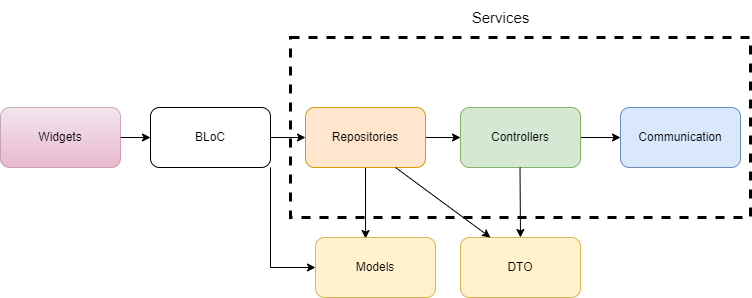
\includegraphics[width=1.0\textwidth]{assets/images/package-scheme.png}
	\caption{Components Dependency}
	\label{fig:package-scheme}
\end{figure}

\newpage

\subsection{Component view}
\label{sec:component}
In the following diagram only the application client is analyzed in detail
\begin{figure}[ht]
\centering
	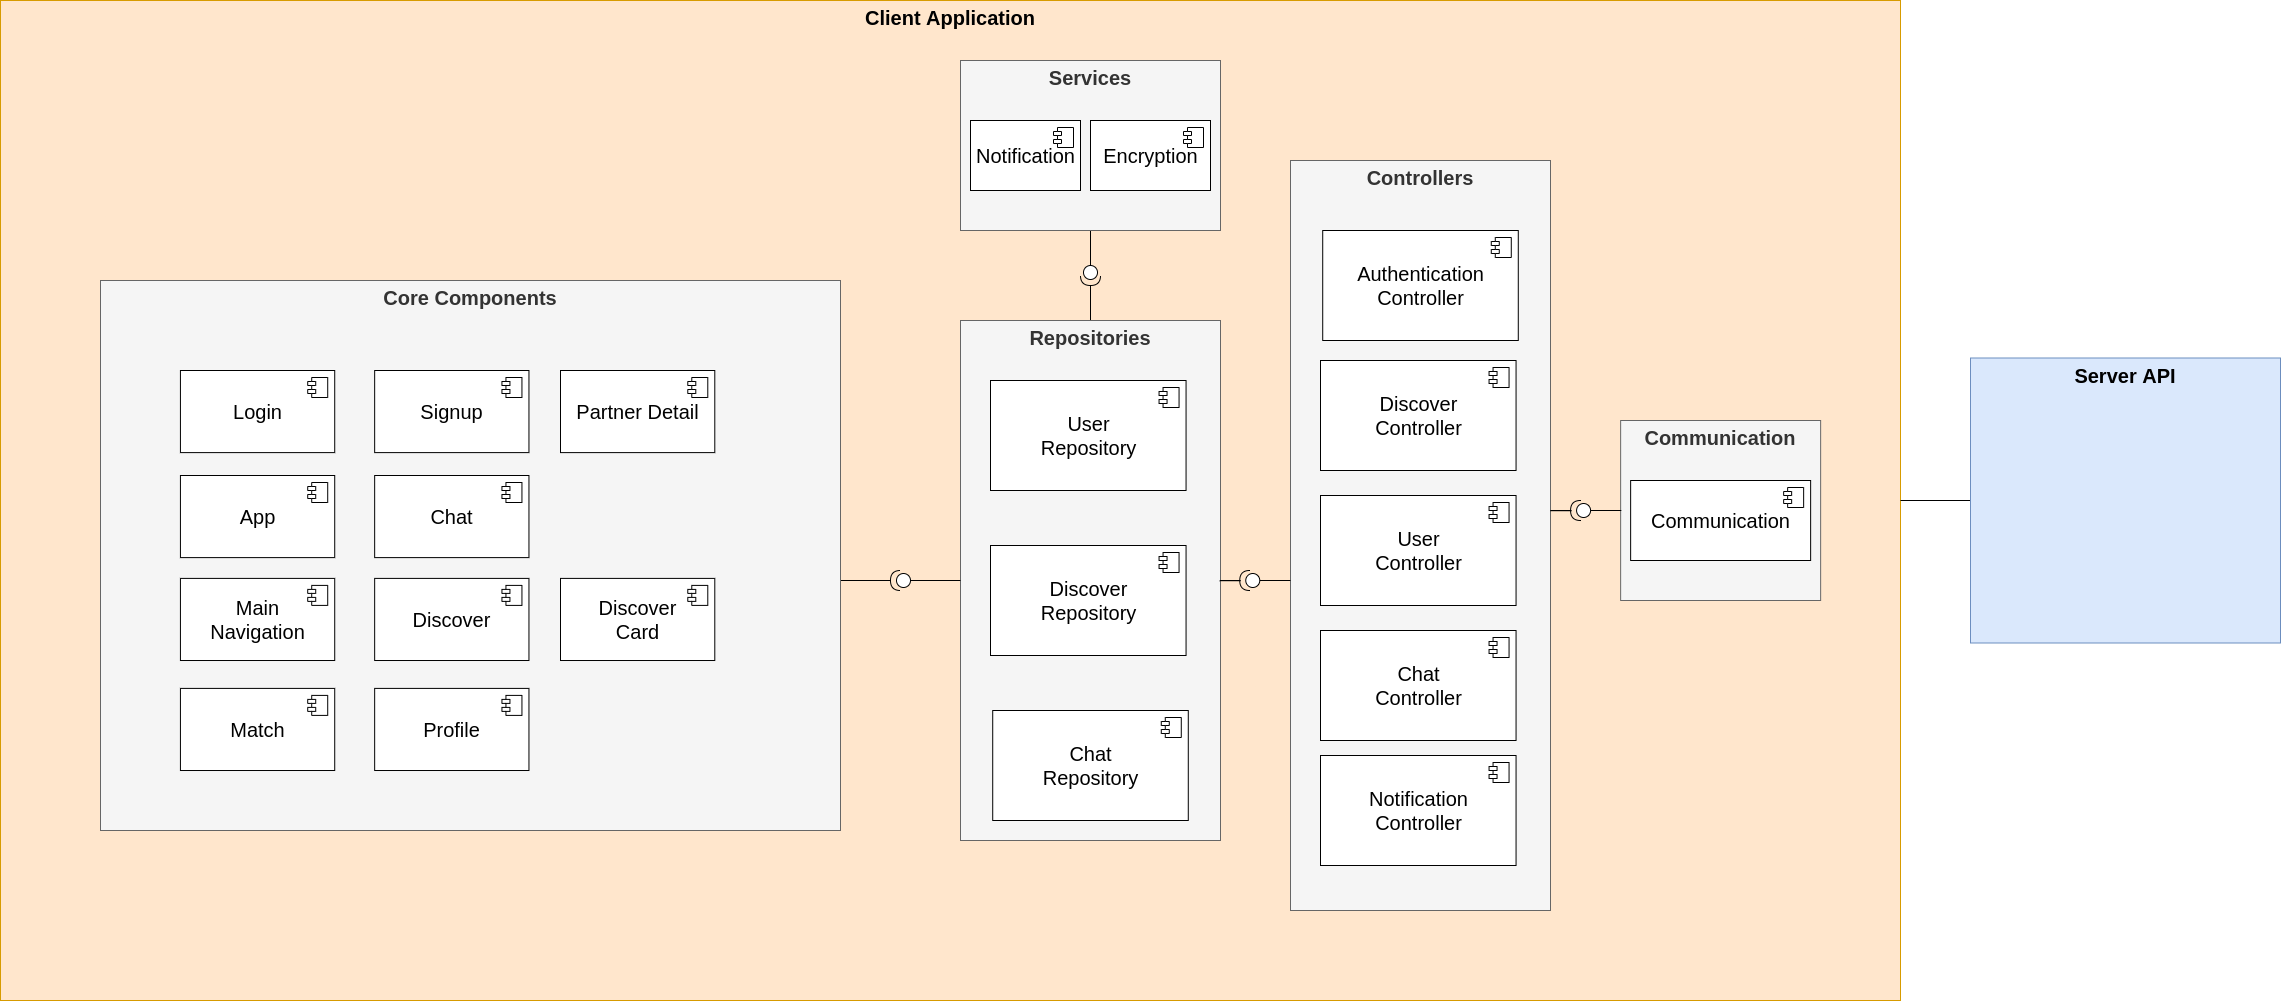
\includegraphics[width=1.0\textwidth]{assets/images/component-view.png}
	\caption{Exapnded Components Dependency}
	\label{fig:component-view}
\end{figure}

\subsubsection{Core Components}
\begin{itemize}
	\item \textbf{AppBloc}: is responsible to show the login page (if the user is not authenticated) or the main screen (otherwhise), this BLoC also store the authenticated user.
	\item \textbf{LoginBloc}: is responsible for the validation of the login credential and the submission of those.
	\item \textbf{SignupBloc}: is responsible for the validation and submission of the user's data.
	\item \textbf{MainBloc}: is responsible for the navigation between the main pages.
	\item \textbf{MatchBloc}: is responsible for keeping the records of the partners liked by the user and the partners that like the user, find the matches.
	\item \textbf{ChatBloc}: is responsible for managing the chats with the messages.
	\item \textbf{DiscoverBloc}: get the possible partners from the repository and handle all the event in the Discover view.
    \item \textbf{DiscoverCardBloc}: is used to mange the single partner to fetch pictures and handle the action inside each discover card.
    \item \textbf{PartnerDetailBloc}: fetch the partner from the given username and put it in its state to be able to display it.
    \item \textbf{ProfileBloc}: handle the changes of the user data, saving them on the server.
\end{itemize}

\subsubsection{Repositories}
\label{sec:repositories}

\begin{itemize}
	\item \textbf{ChatRepository}: is used to get and send messages.
	\item \textbf{DiscoverRepository}: is used to fetch all the data reguarding the partners, unencrypt everything that can be unencrypted, put like (send add like message), put dislike (send remove like message), and receive like message.
	\item \textbf{UserRepository}: is used for the authentication, fetch and edit of all the data related to the user of the app.
\end{itemize}

\subsubsection{Controllers}
\label{sec:controllers}
\begin{itemize}
	\item \textbf{AuthenticationController}: Handles everything is needed in the signup, login phases.
	    \begin{itemize}
	        \item \textit{ SignUp:} Register a user into the system using a username and a public key.
	        \item \textit{ GetLoginChallenge:} Returns a login challenge for a given username.
	        \item \textit{ LogIn:} Logs a user into the system using the username and the login challenge
	        \item \textit{ LogOut:} Logs a user out from the system.
	    \end{itemize}
	\item \textbf{ChatController}: Exposes a single API for send a message to a user.
		\begin{itemize}
	        \item \textit{ SendMessage:} Send a message (string) to a user using the username. It's assumed that the user is already logged in (i.e. in the current RESTful implementation, a valid JWT is sended with the request).
	    \end{itemize}
	\item \textbf{DiscoverController}: Exposes all APIs for fetching other users data.
		\begin{itemize}
	        \item \textit{ FetchPartners:} given some filtering options (for example the number of results), returns a list of possible partners for the logged user, according to his public searching criteria.
	        \item \textit{ FetchPartner:} Returns all user info from the username, with the exception of the images' content.
	        \item \textit{ SendSealedLikeMessage:} Sends a like message to a user.
	        \item \textit{ FetchPartnerPublicPicture:} Fetches a public image content of a user by the name.
	        \item \textit{ FetchPartnerEncryptedPrivatePicture:} Fetches a private image content of a user by the name.
	        \item \textit{ FetchPublicKey:} Gets the public key of a user by the username.
	    \end{itemize}
	\item \textbf{NotificationsController}: Exposes a single method to fetch a notification. A notification could be a like message or a chat message. Basically it's everything the server needs to to client:
		\begin{itemize}
				\item \textit{ Fetch:} Waits asynchronously until a new notification is available, and returns it back.
		\end{itemize}
	\item \textbf{UserController}: Handles everything is related to the logged user.
	\begin{itemize}
    	    \item \textit{ FetchUser:} Fetch all the logged user data.
	        \item \textit{ PushUser:} Updates all the logged user data.
	        \item \textit{ PushPublicPic:} Adds a public picture to the user profile.
	        \item \textit{ FetchPublicPics:} Fetches all specified public images contents from the logged user.
	        \item \textit{ PushEncryptedPrivatePic:}: Adds a private picture to the user profile.
	        \item \textit{ FetchEncryptedPrivatePics:} Fetches all specified private images contents from the logged user.
	        \item \textit{ FetchSymmetricEncryptedKeys:}: Fetches all symmetric keys used by the user until his registration.
	        \item \textit{ PushSymmetricEncryptedKeys:} Adds a symmetric key to the keys collection of the user.
	\end{itemize}
	
\end{itemize}
The controller package has also associated a models folder with the DTOs that are used for the transfer of data to and from the server. \\
Each controller has two implementation, one that exploit the Communication package to communicate with the server and one that simply mock those function for testing purpose. 

\subsubsection{Other Services}
\label{sec:services}
\begin{itemize}
    	    \item \textbf{EncryptionService} \\ It is compose by two separate services:
			\begin{itemize}
				\item \textbf{SymmetricEncryption} \\
					Is a AES implementation that generates random keys and encrypt and decrypt data.
				\item \textbf{AsymmetricEncryption} \\
					Is an RSA implementation that generates a pair of key and encrypt, decrypt, sign and verify data.
			\end{itemize}
\end{itemize}

\subsubsection{Communication}
\label{sec:communication}
The communication interfaces exposes the following methods:
\begin{itemize}
    	    \item \textbf{ Post:} Post an object to and endopoint (with authentication if needed), and returns back the raw response.
	        \item \textbf{ Get:} Returns back an object from an endpoint specifying some query parameters (with authentication if needed).
	        \item \textbf{ Download:} Downloads a raw file (i.e. an iamge) from a specified endpoint (with authentication if needed).
	        \item \textbf{ SetToken:} Sets an access token for all next requests.
	        \item \textbf{ UnsetToken:}: Remove the access token for all next requests.
\end{itemize}

\subsubsection{Server}	
\label{sec:server}
The Server is based on the Clean Architecture of Jason Taylor together with CQRS pattern. It's composed of 4 projects: 
\begin{itemize}
	        \item \textbf{ Domain:} Contains all the domain models. In this project there is the very core of the application. There is no logic at all here.
	        \item \textbf{ Application:} This project references only the Domain project. Contains all the business logic of the application and defines all the interfaces of the services needed. However in this project there are not the implementation of these services.
	        \item \textbf{ Infrastructure:} References the Domain and the Application projects. Contains all the implementation of the services defined in the Application layer. For example, While the application layer contains an interface \textit{IUserCrud} containing all the methods for create, update, delete and update a user, the implementation of this interface is contained here in the infrastructure project. The diea behind that is to be able to plug in and out different infrastructure layers for the same application projects without any modification
    	    \item \textbf{ Server:} This is a Asp.Net 6.0 MVC Web Application, where controllers contains the REST endpoints. Authentication is implemented with Json Web Token together with the standard Claims-based authentication of ASP.NET Core. This project references all the other projects but the only reason why the infrastructure project is referenced is to bind Application level interfaces to Infrastructure implementations in the dependency injection container at the startup. In this project are defined all the DTOs, that are mapped to the other projects in domain models and/or queries/commands.
\end{itemize}
CQRS is implemented trough the NuGet package MediatR. This, together with the dependency injection and the Clean Architecture offers great decoupling and testability.
\newpage
\subsection{Runtime view}
\label{sec:runtime-view}
In this section are shown the sequence diagrams of some features. They are useful to clarify the runtime behaviour of the components involved for the main functionalies
\subsubsection{Put like}
\begin{figure}[ht]
	\centering
		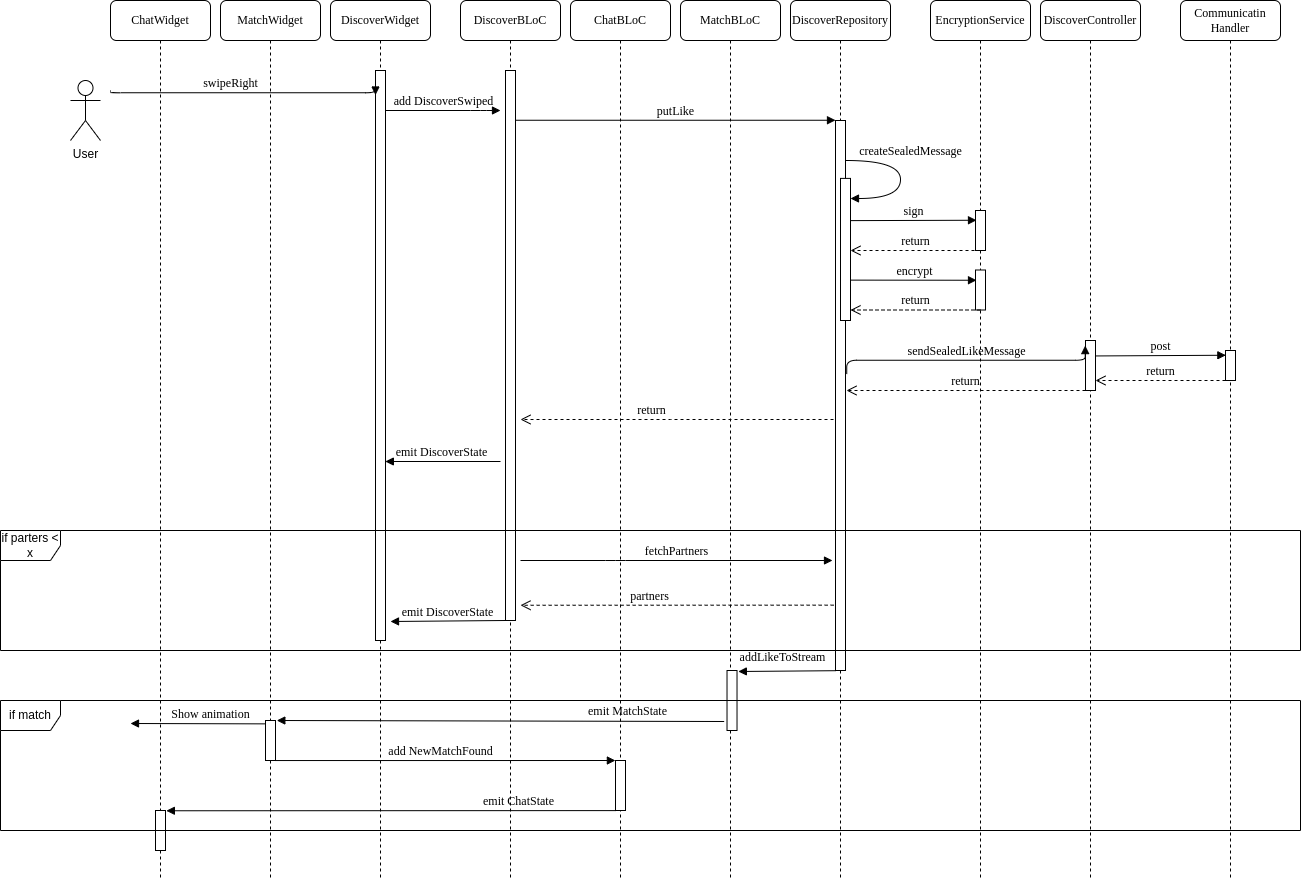
\includegraphics[width=1.0\textwidth]{assets/images/put-like-sequence.png}
		\caption{Put like sequence diagram}
		\label{fig:put-like-sequence}
\end{figure}
\newpage
\subsubsection{Signup}
\begin{figure}[ht]
	\centering
		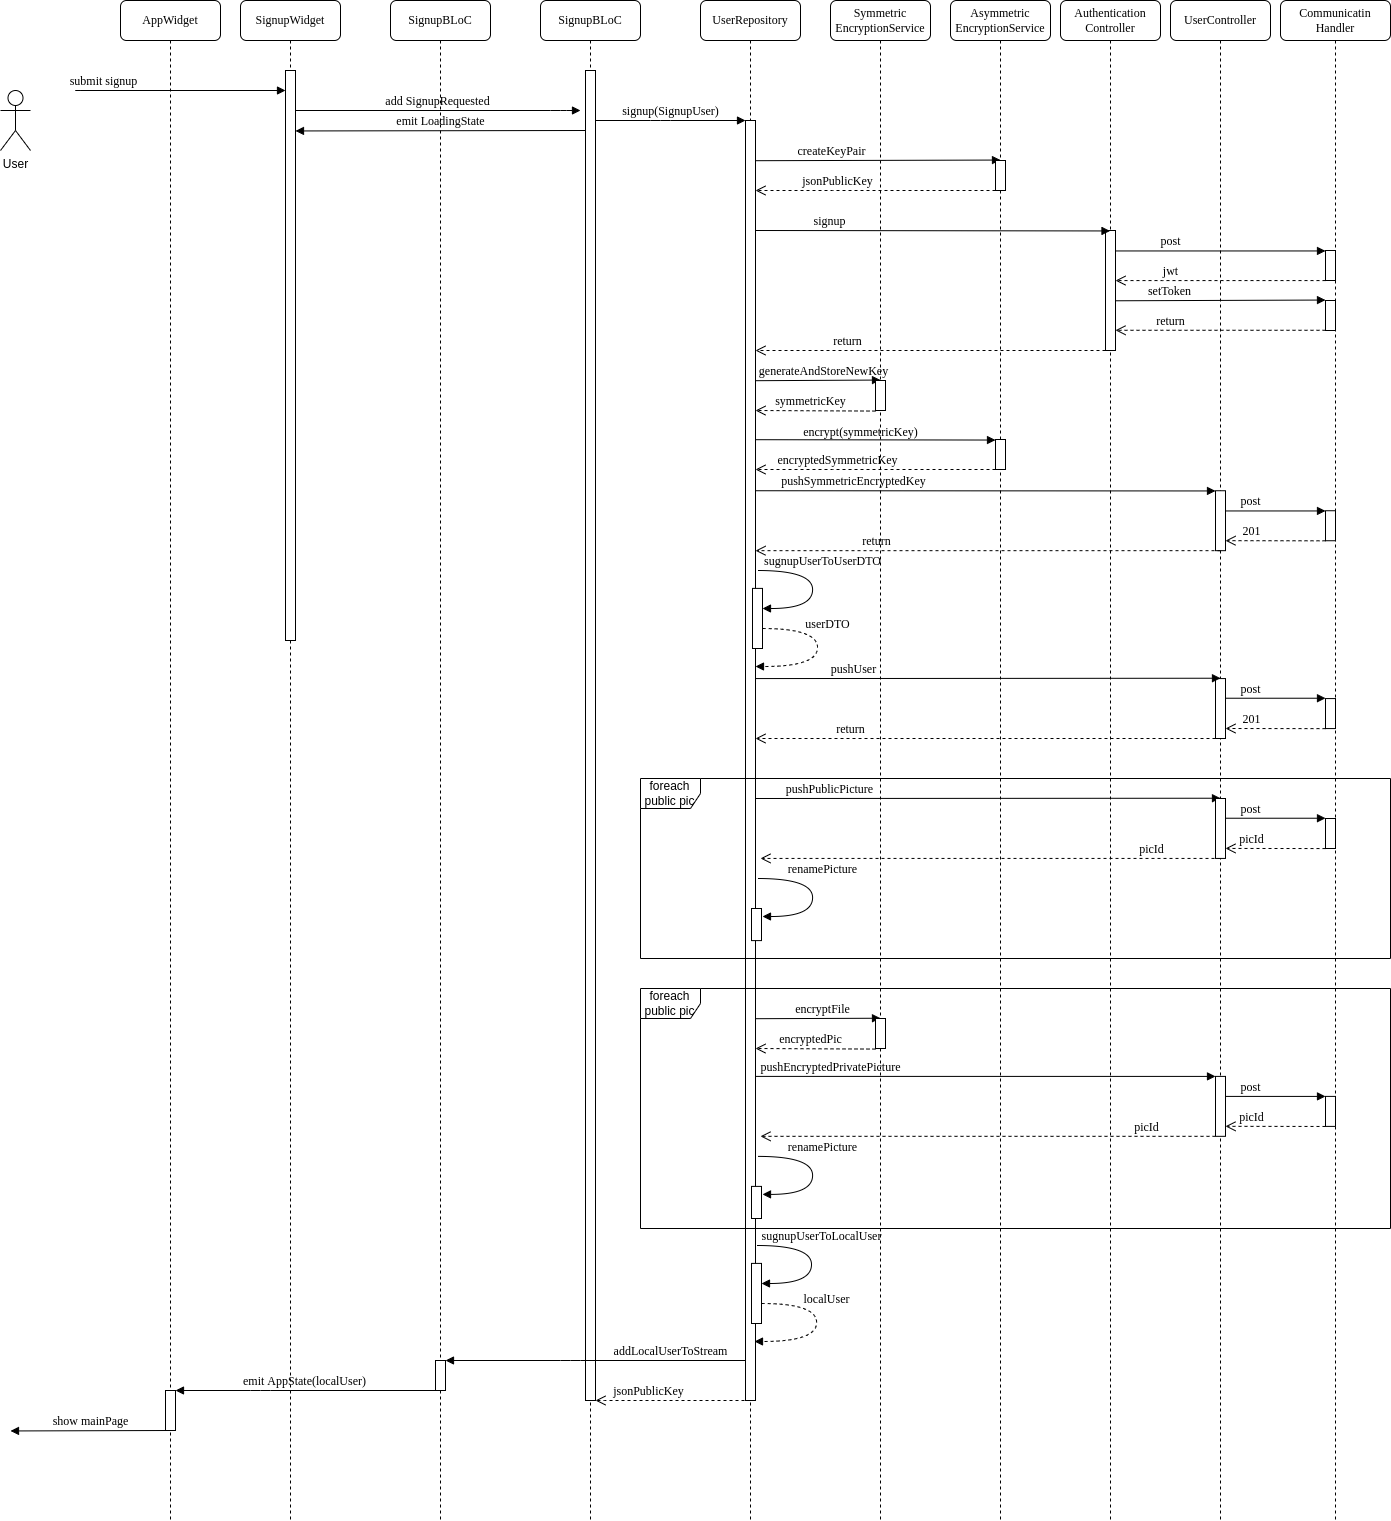
\includegraphics[width=1.0\textwidth]{assets/images/signup-sequence.png}
		\caption{Signup sequence diagram}
		\label{fig:signup-sequence}
\end{figure}
\newpage
\subsection{Selected architectural styles and patterns}
\begin{itemize}
	\item \textbf{BLoCs}: A state mangement solution. \\
		We organized the code in BLoCs (Business Logic Components) to decople the UI logic for presentation and all the business logic and state of the app.
	
	\item \textbf{DTOs Pattern}: Data Transfer Objects. \\
		The communication between the the server and the user application uses DTOs so that if the sever API will change the client has to update only the DTOs and not the model.
		
	\item \textbf{DI Pattern}: Dependency injection. \\
		We follow the DI Pattern to separate the concerns of constructing objects and using them. 
		This way ensures that an object or function which wants to use a given service should not have to know how to construct those services.
		A great advantage is also noticable in writing tests because it's really easy to mock and inject a class dependecies.
		
	\item \textbf{RESTful architecture}: REST is a software architectural style. \\
		The communication between the server and the user application uses HTTP(S) requests which follows REST principles.
		One of the most important REST principles is that the interaction between the client and server is stateless between requests. Each request from the client to the server must contain all of the information necessary to understand the request. For instance the client wouldn’t notice if the server were to be restarted at any point between the requests.
		This is achieved using a uniform and predefined set of stateless operations based on strict use of HTTP request types.
	
\end{itemize}

\newpage

\subsection{Other design decisions}

\subsubsection{Encryption Protocol}
To garantee the privacy of the user we created a protocol to minimize the knowledge of the server. 
\begin{itemize}
	\item Every user have an asymmetric key pair generaetd from the username and password that garantee their identity.
	\item All the private data of a user is encrypted with a randomly generated symmetric key before been send to the server.
	\item When a user (Alice) want to put a like to another user (Bob), it create a sealed message to send to Bob in this way:
		\begin{itemize}
			\item Sign Bob's username with her private key.
			\item Create a PackedMessage with: the signed username, the list of symmetric key used for the private data and Alice's username.
			\item Encrypt the PackedMessage with Bob's public key.
		\end{itemize}
	\item When Bob receive a like message, he decrypt the message with his private key, verify that his own username is signed by Alice, store the symmetric keys that will use to decrypt the private data.
\end{itemize}

\newpage

\section{User interface design}
\label{sec:UI}


\subsection{UX Diagrams}
In all the diagrams the actions to go back are omitted to simplify the diagrams.
The UX is slightly different for tablet and smartphone to reach a better experience.

\begin{itemize} 
	\item \bf Smartphone
		\begin{figure}[!htb]
			\centering
			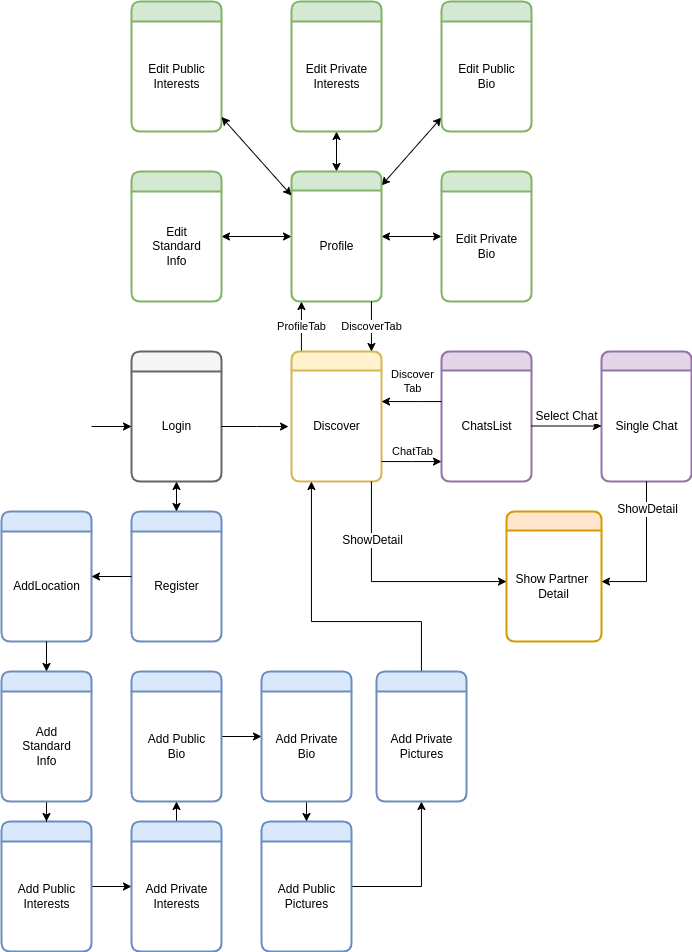
\includegraphics[width=0.8\textwidth]{assets/images/UX.png}
			\caption{Phone UX diagram}
		\end{figure}

	\newpage
	\item \bf Tablet
		\begin{figure}[!htb]
			\centering
			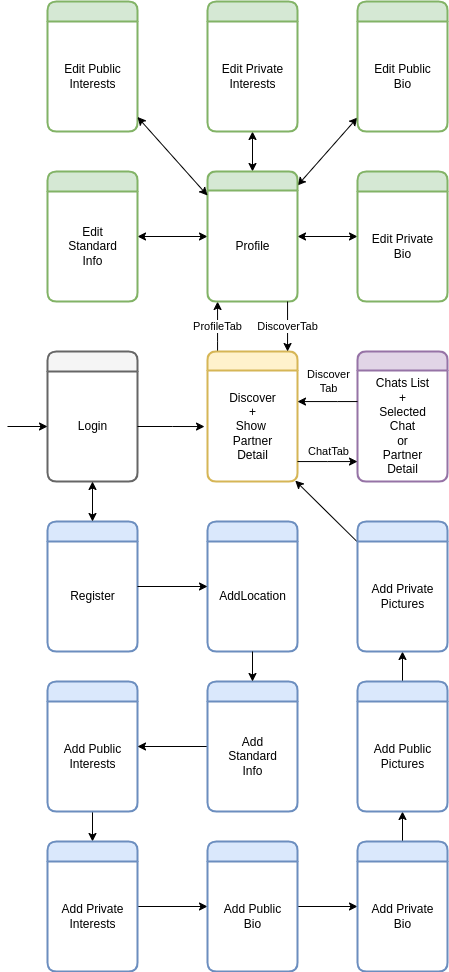
\includegraphics[width=0.6\textwidth]{assets/images/UX-tablet.drawio.png}
			\caption{Tablet UX diagram}
		\end{figure}

\end{itemize} 

\clearpage
\subsection{User interface}

\subsubsection{Authentication}
\begin{figure}[!htb]
	\centering
	\begin{minipage}{.45\textwidth}
		\centering
		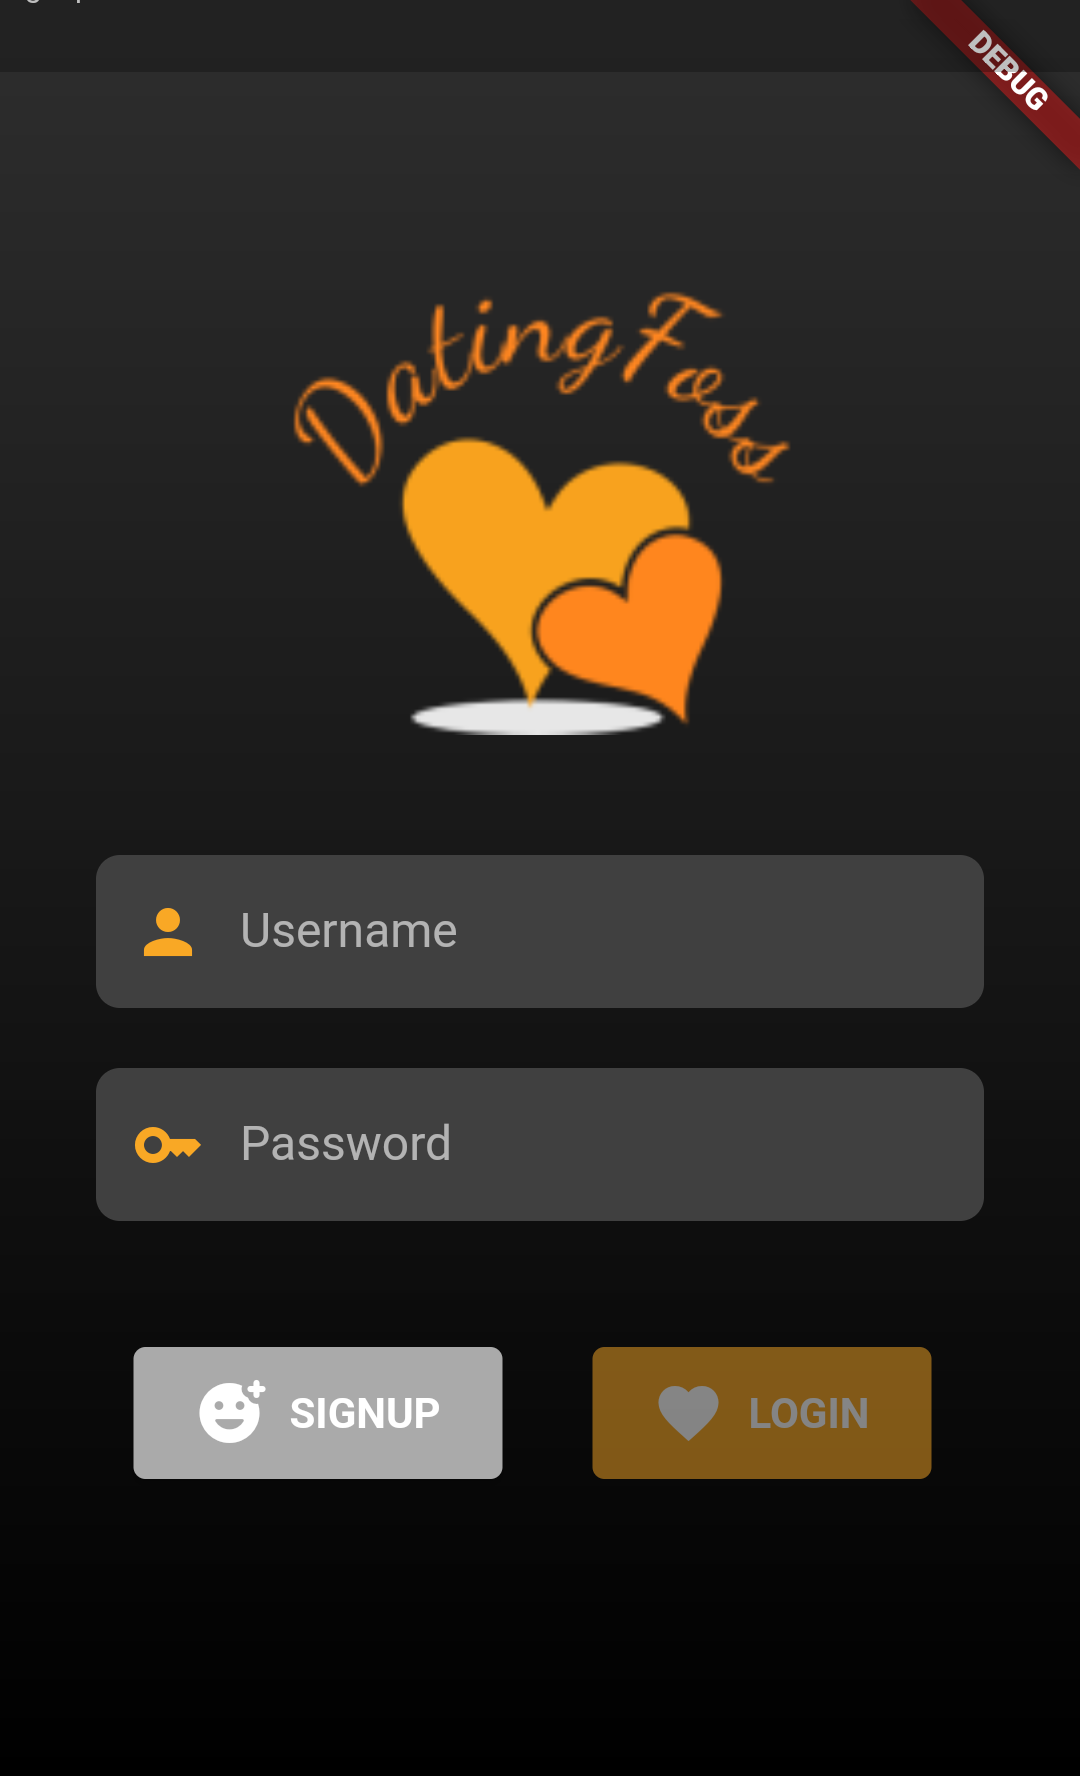
\includegraphics[height=7cm,keepaspectratio]{assets/images/ui/signup/00-login.png}
		\caption{Login}
	\end{minipage}\quad
	\begin{minipage}{.45\textwidth}
		\centering
		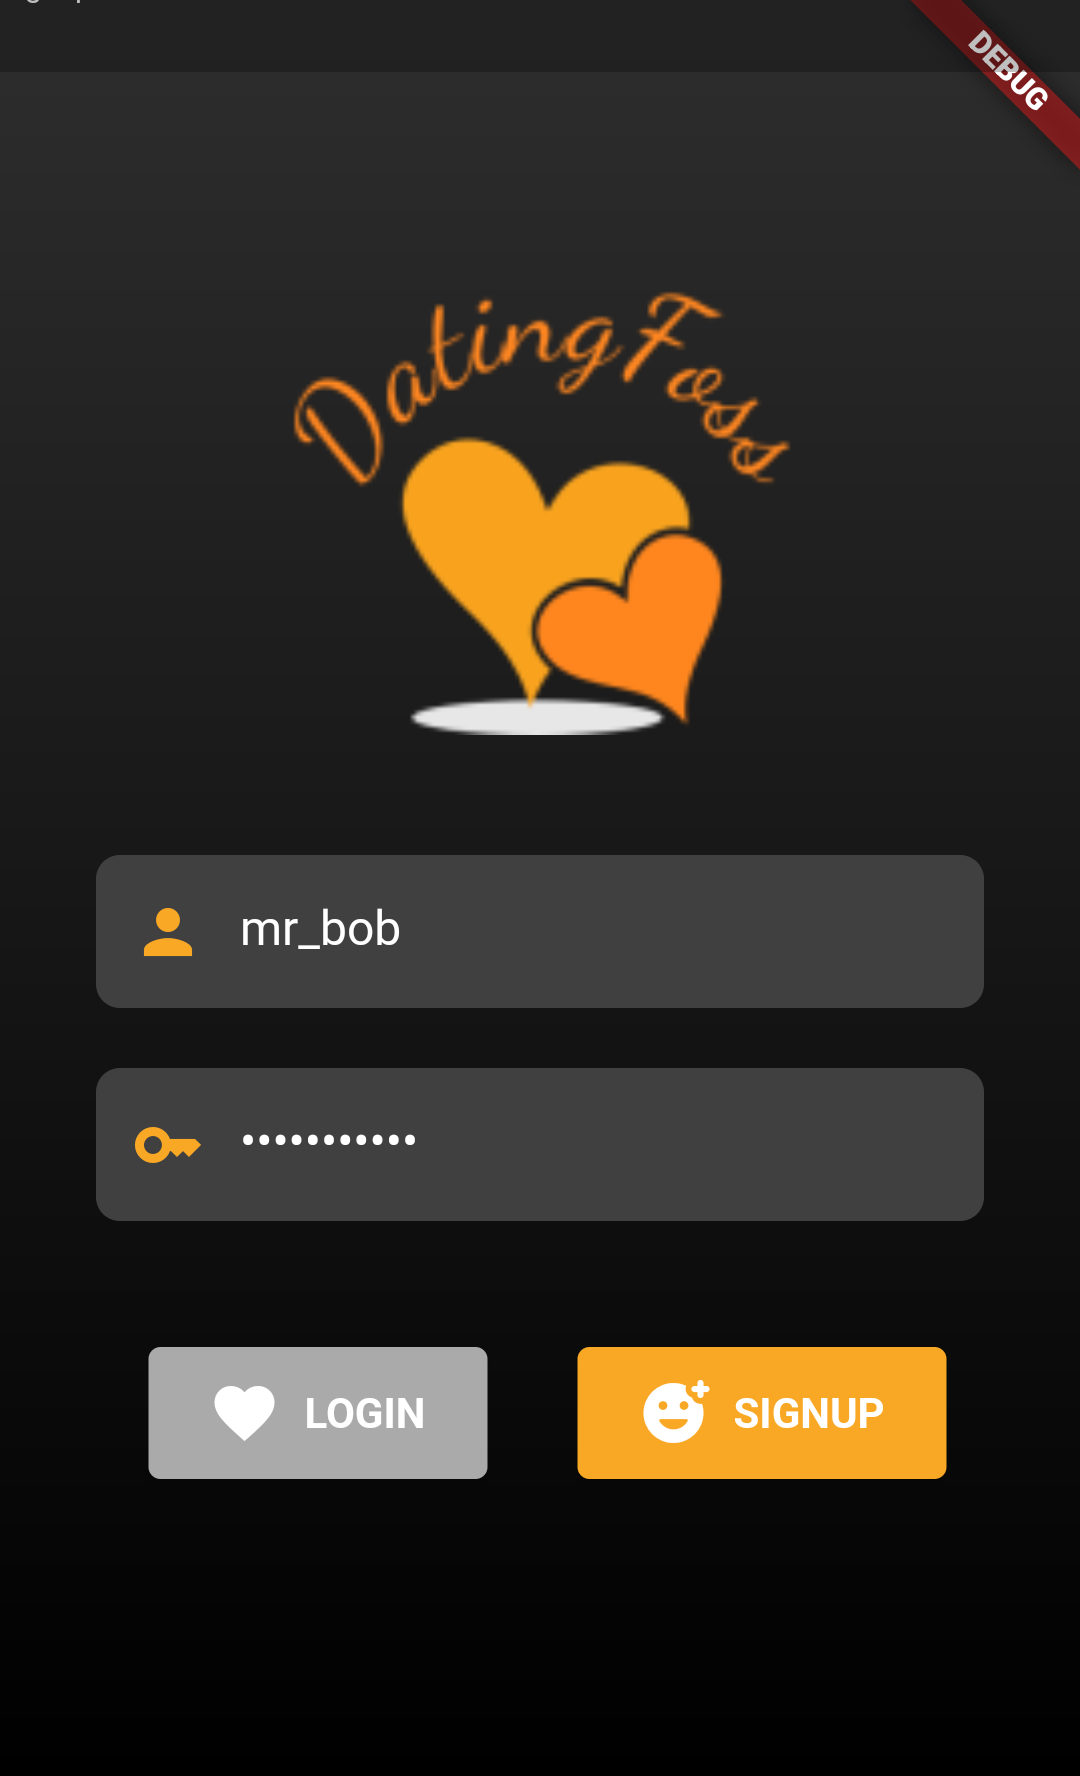
\includegraphics[height=7cm,keepaspectratio]{assets/images/ui/signup/02-signup-filled.png}
		\caption{Signup}
	\end{minipage}
\end{figure}
\begin{figure}[!htb]
	\centering
	\begin{minipage}{.45\textwidth}
		\centering
		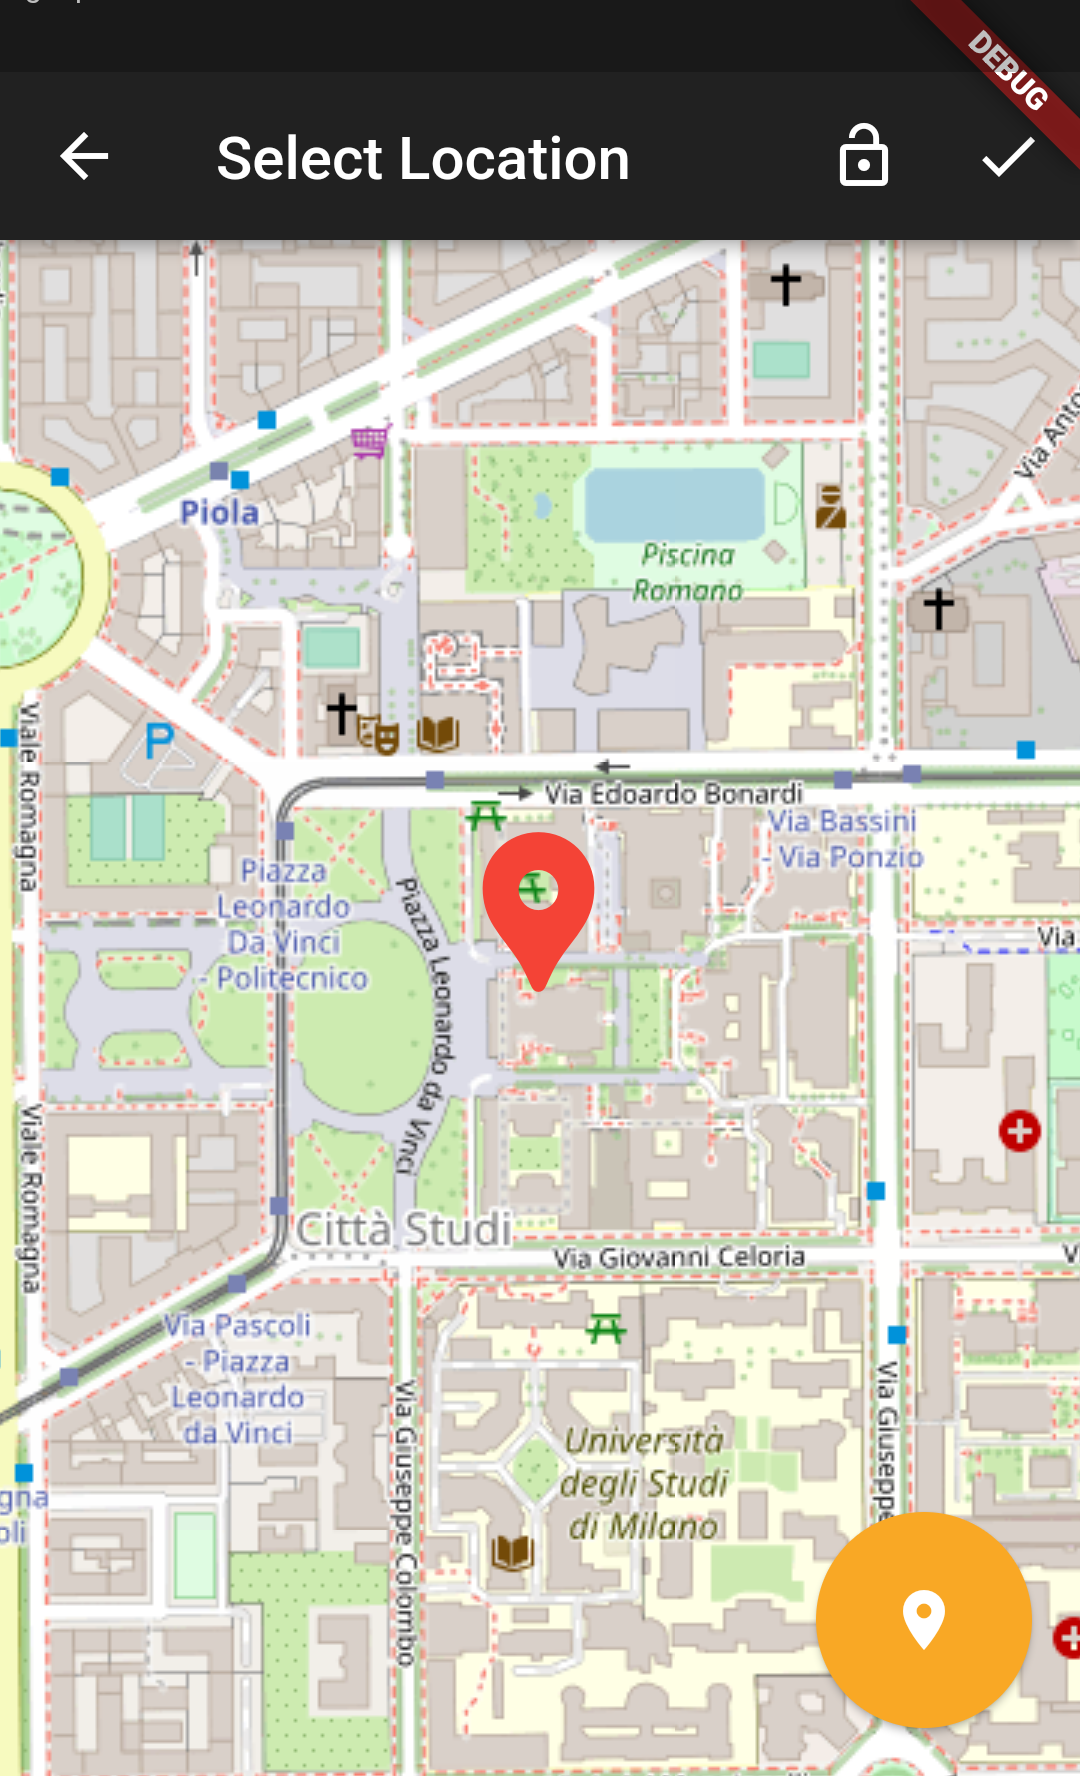
\includegraphics[height=7cm,keepaspectratio]{assets/images/ui/signup/03-map.png}
		\caption{Location}
	\end{minipage}\quad
	\begin{minipage}{.45\textwidth}
		\centering
		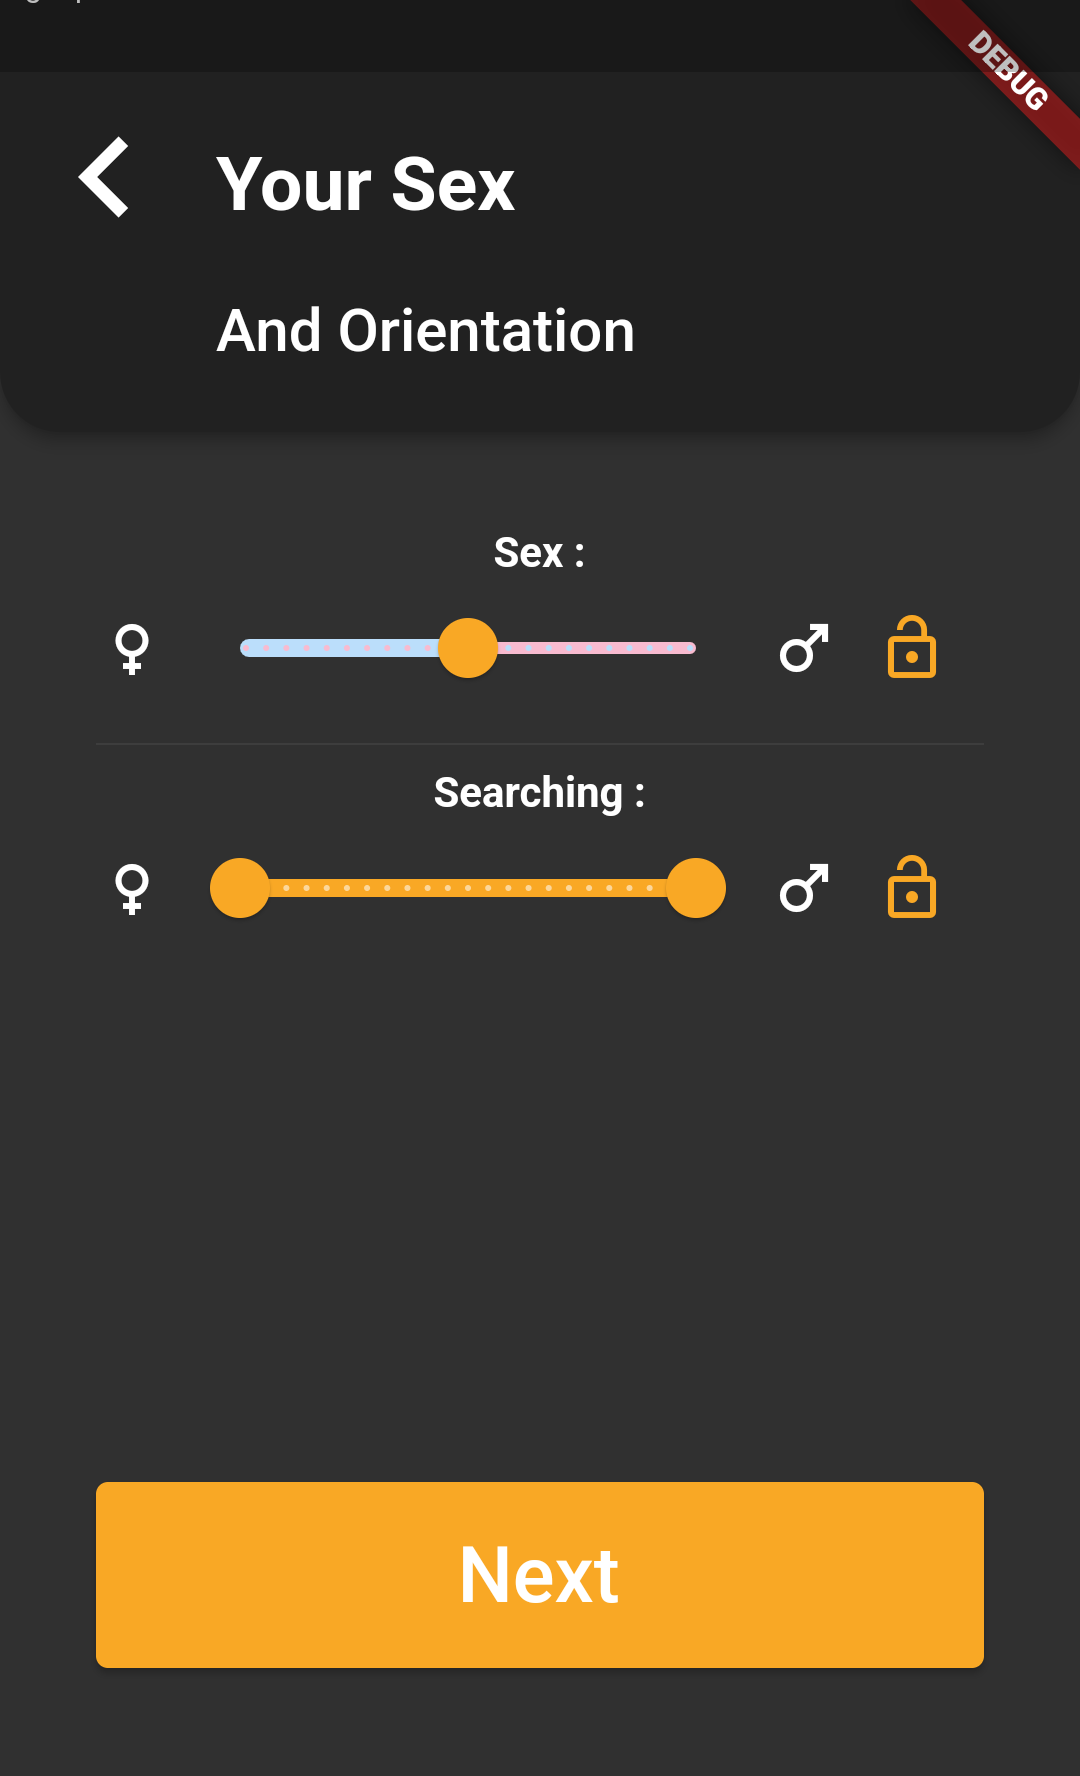
\includegraphics[height=7cm,keepaspectratio]{assets/images/ui/signup/04-sex-and-orientation.png}
		\caption{Sex and Orientation}
	\end{minipage}
\end{figure}
\begin{figure}[!htb]
	\centering
	\begin{minipage}{.45\textwidth}
		\centering
		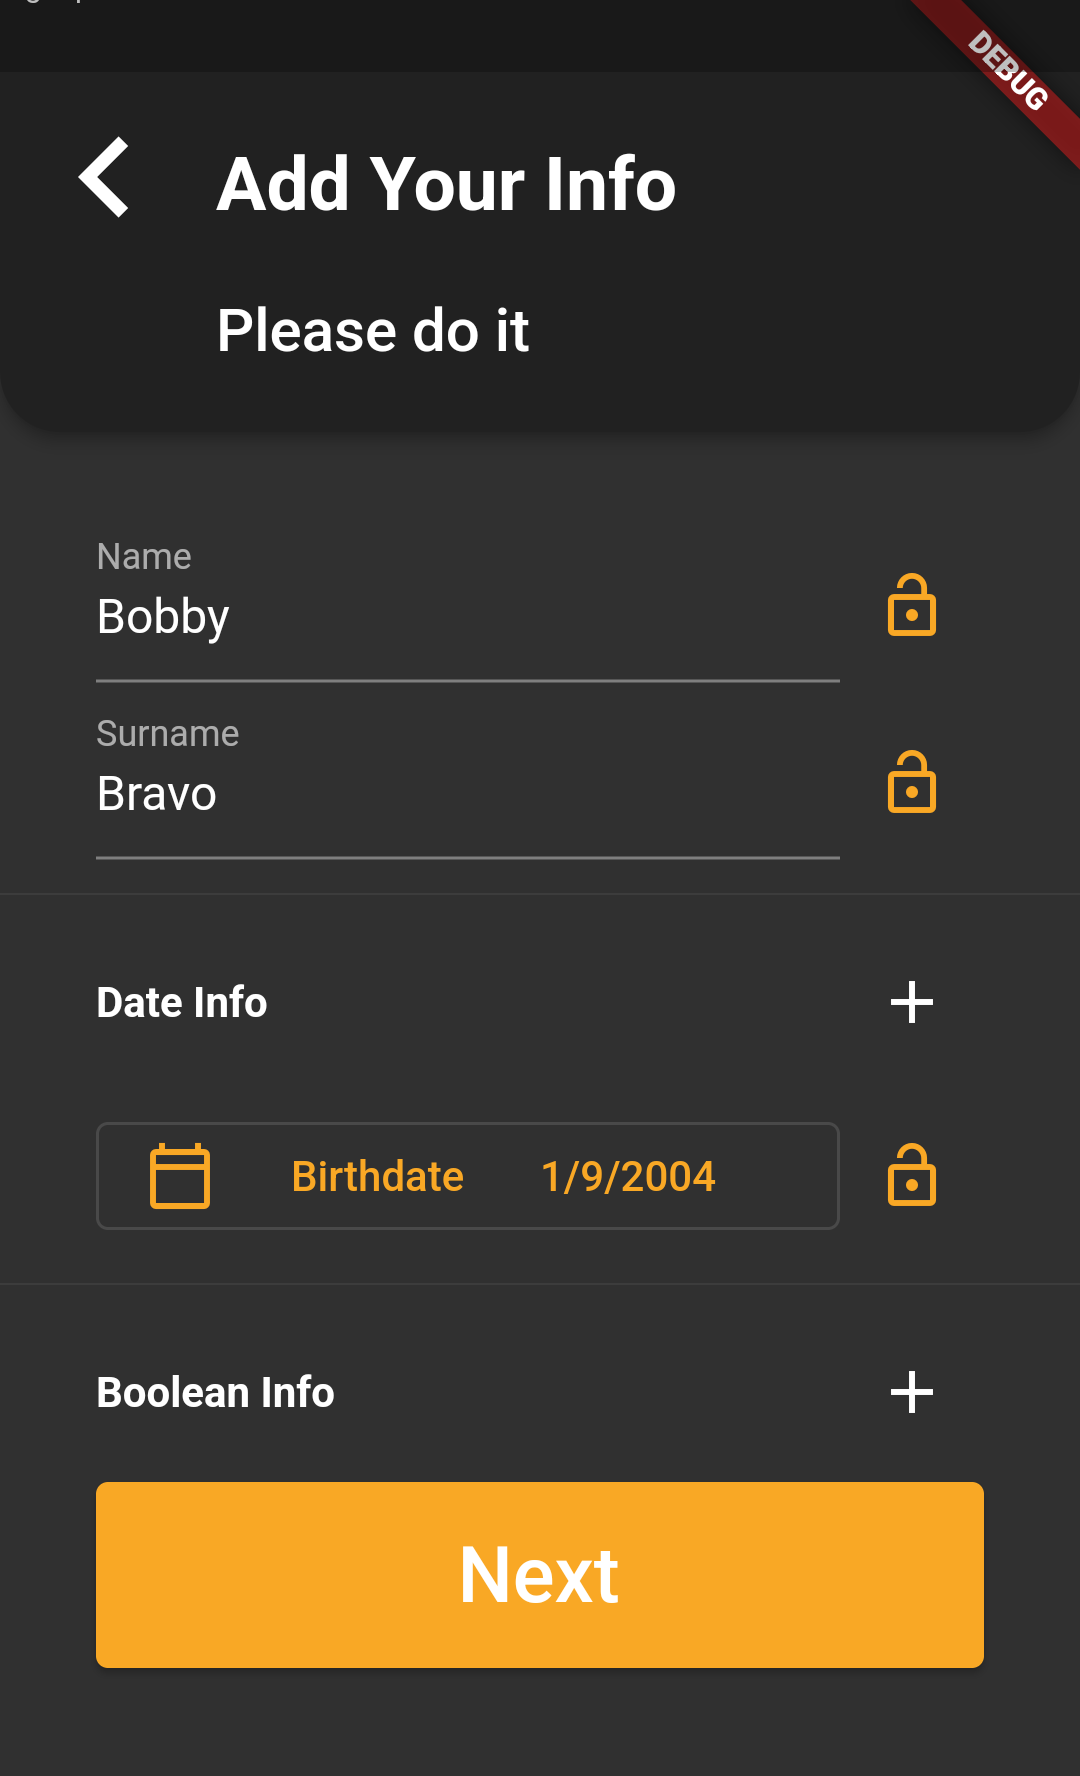
\includegraphics[height=7.7cm,keepaspectratio]{assets/images/ui/signup/07-standard-info-date.png}
		\caption{Standard Info Top}
	\end{minipage}\quad
	\begin{minipage}{.45\textwidth}
		\centering
		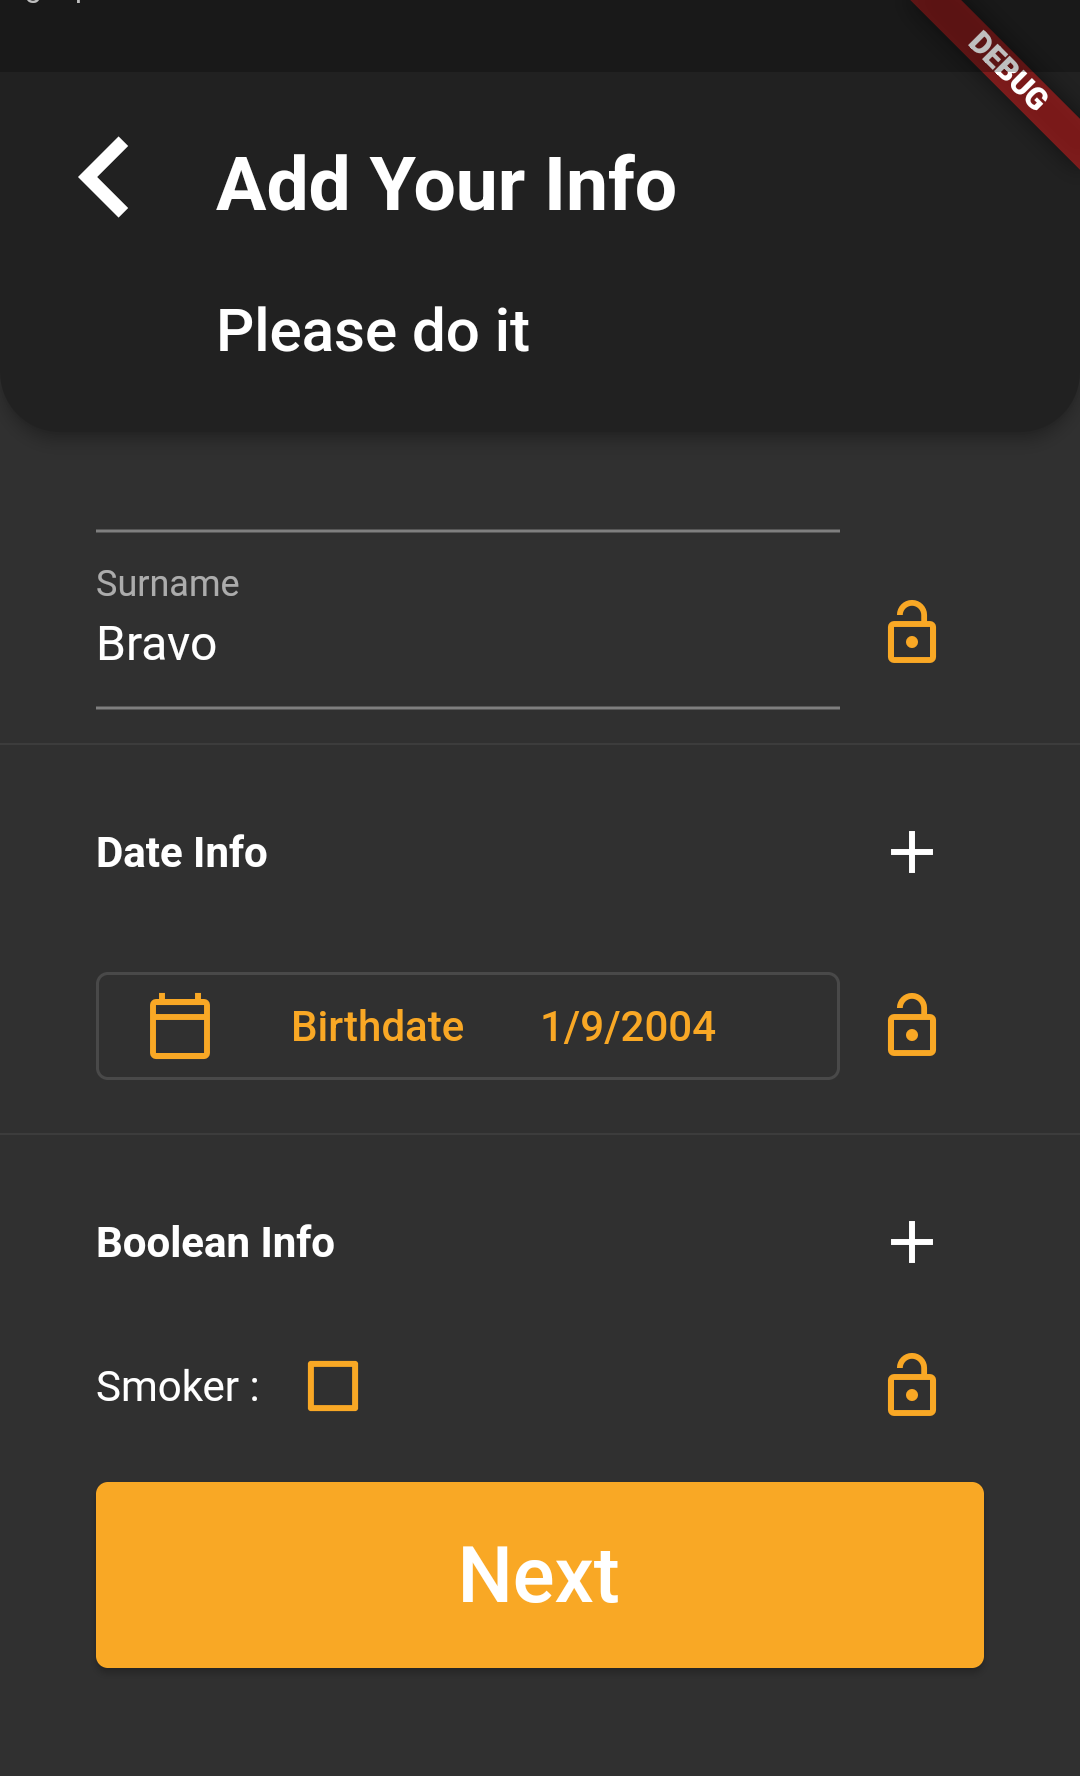
\includegraphics[height=7.7cm,keepaspectratio]{assets/images/ui/signup/08-standard-info-bool.png}
		\caption{Standard Info Bottom}
	\end{minipage}
\end{figure}
\begin{figure}[!htb]
	\centering
	\begin{minipage}{.45\textwidth}
		\centering
		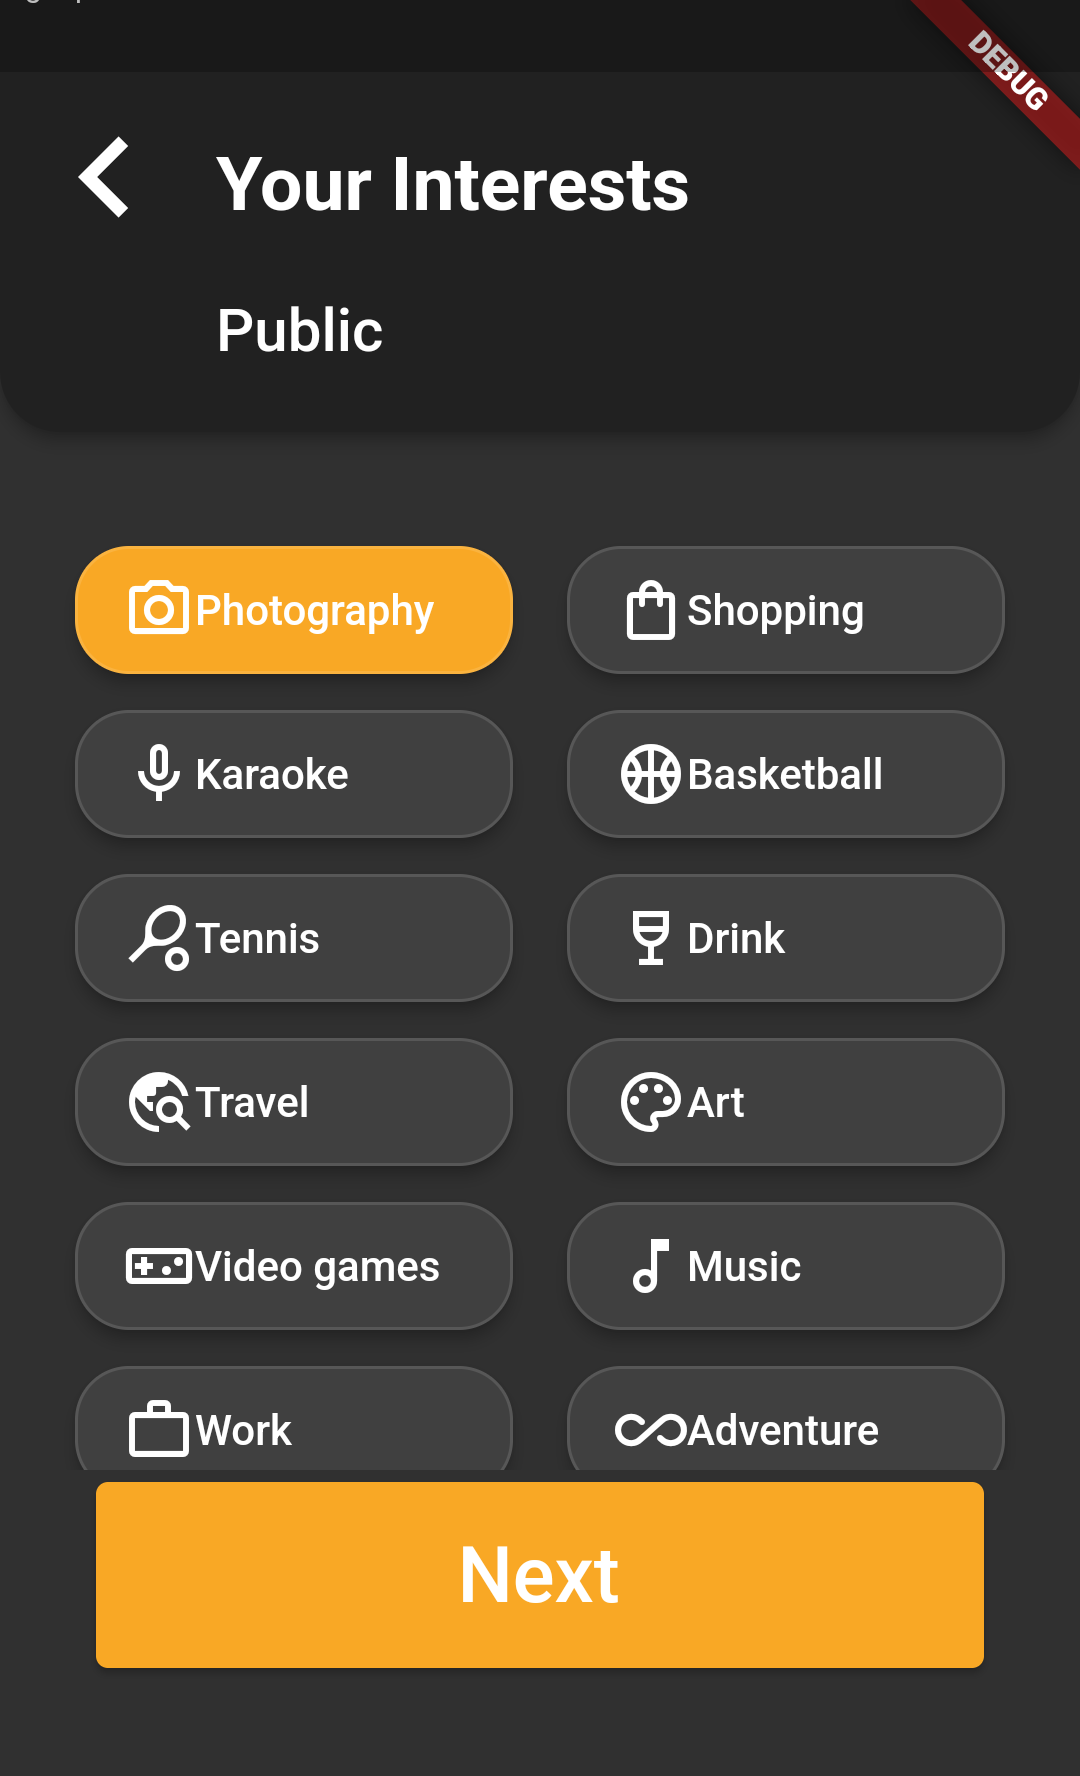
\includegraphics[height=7.7cm,keepaspectratio]{assets/images/ui/signup/10-public-interest-selected.png}
		\caption{Public Interests}
	\end{minipage}\quad
	\begin{minipage}{.45\textwidth}
		\centering
		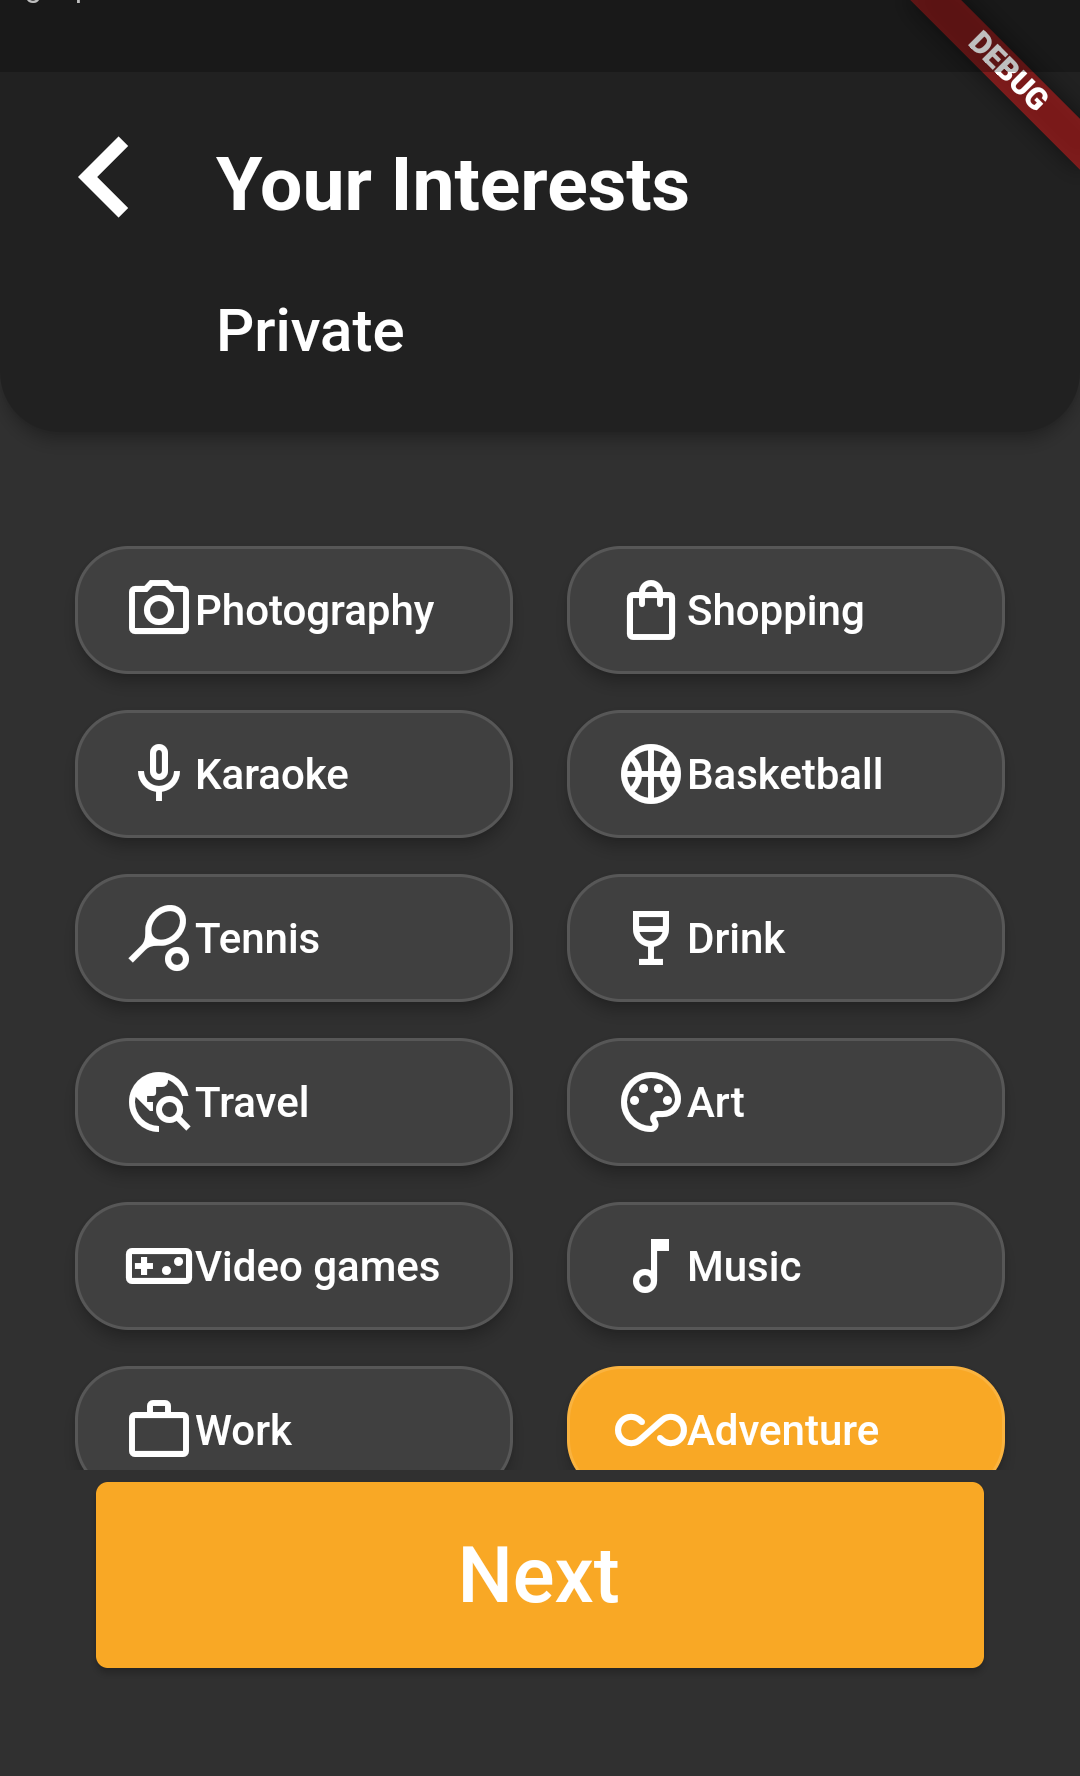
\includegraphics[height=7.7cm,keepaspectratio]{assets/images/ui/signup/12-private-interest-selected.png}
		\caption{Private Interests}
	\end{minipage}
\end{figure}

\begin{figure}[!htb]
	\centering
	\begin{minipage}{.45\textwidth}
		\centering
		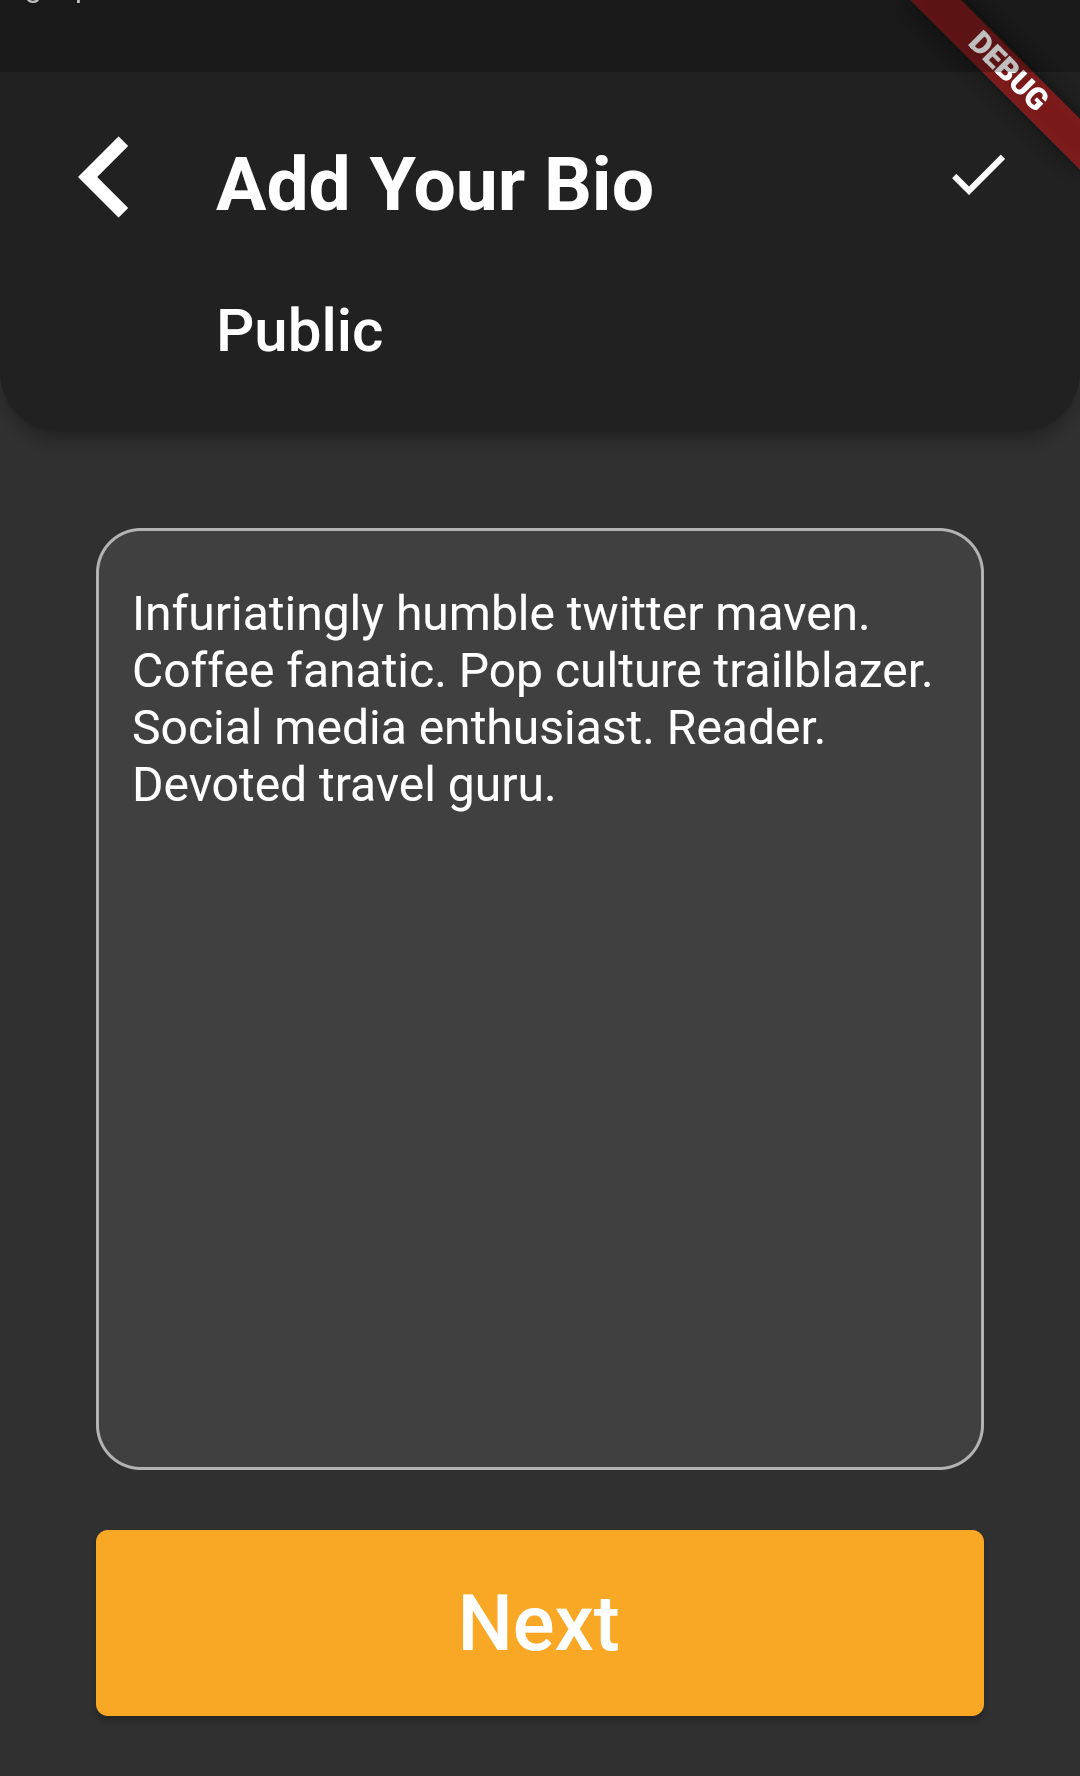
\includegraphics[height=7.7cm,keepaspectratio]{assets/images/ui/signup/14-public-bio-selected.png}
		\caption{Public Bio}
	\end{minipage}\quad
	\begin{minipage}{.45\textwidth}
		\centering
		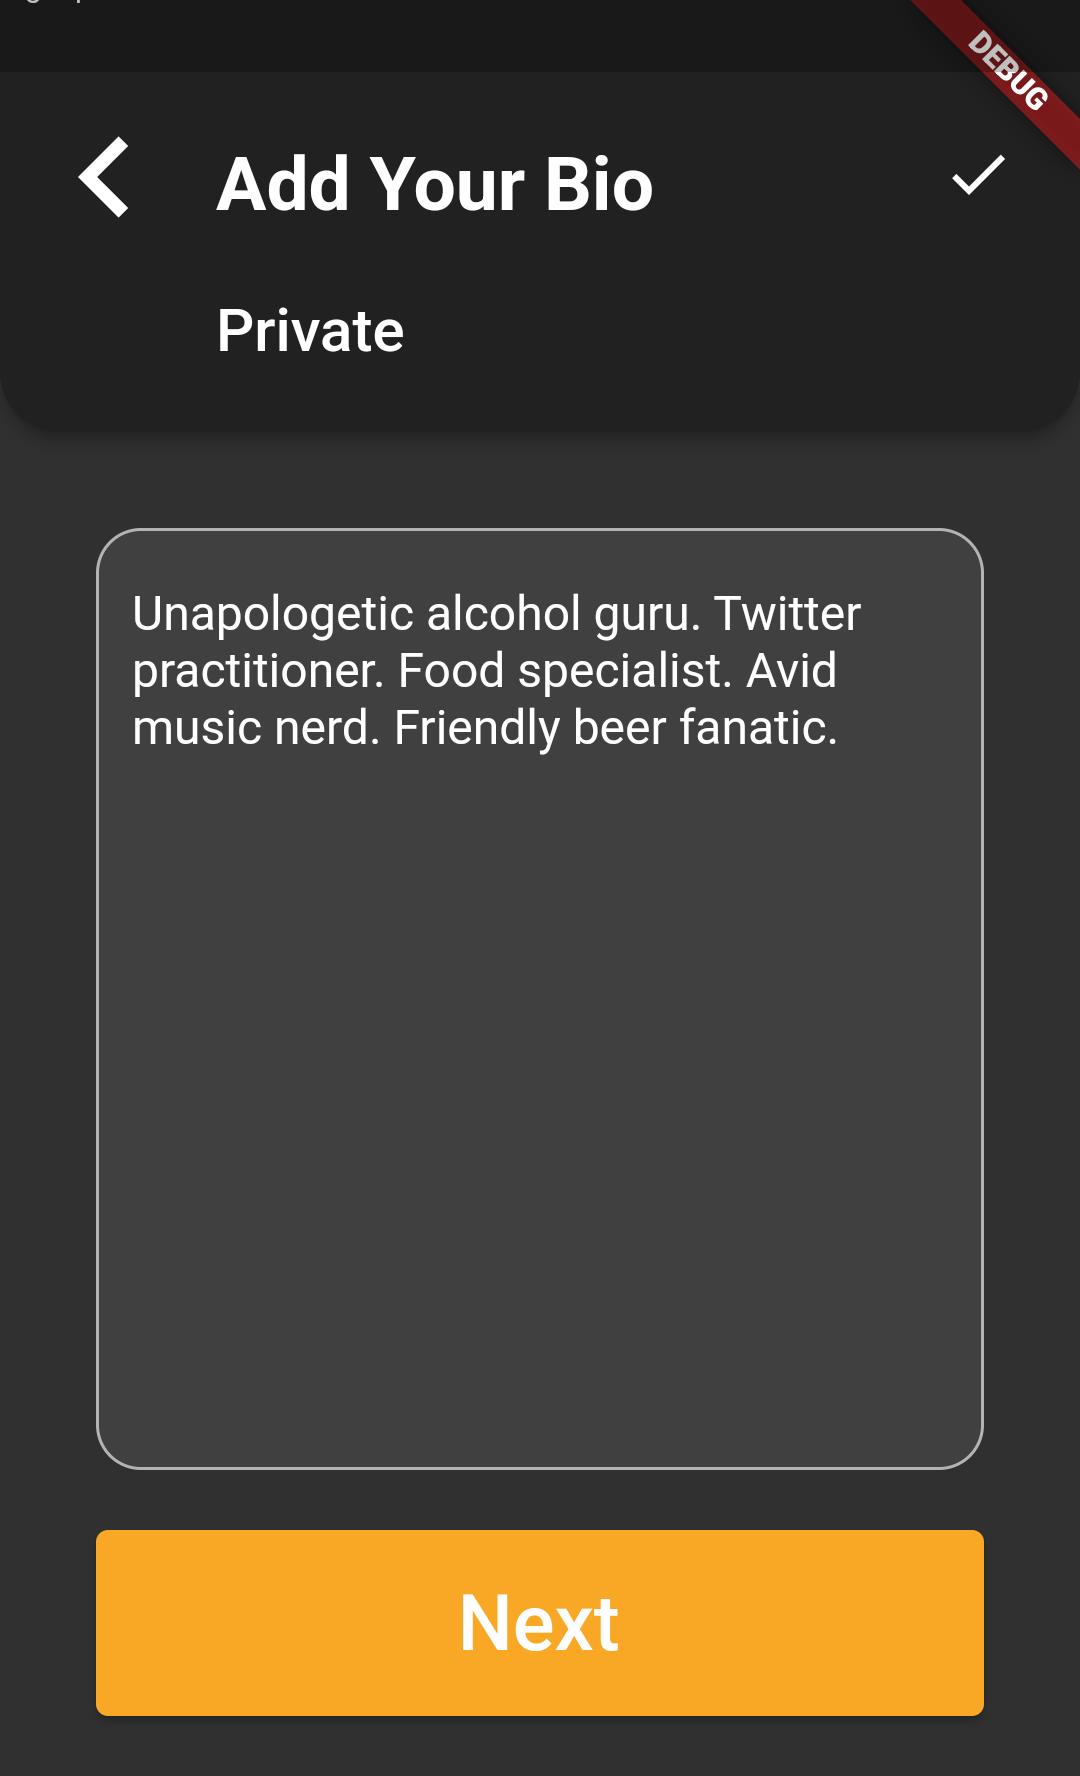
\includegraphics[height=7.7cm,keepaspectratio]{assets/images/ui/signup/16-private-bio-selected.png}
		\caption{Private Bio}
	\end{minipage}
\end{figure}
\begin{figure}[!htb]
	\centering
	\begin{minipage}{.45\textwidth}
		\centering
		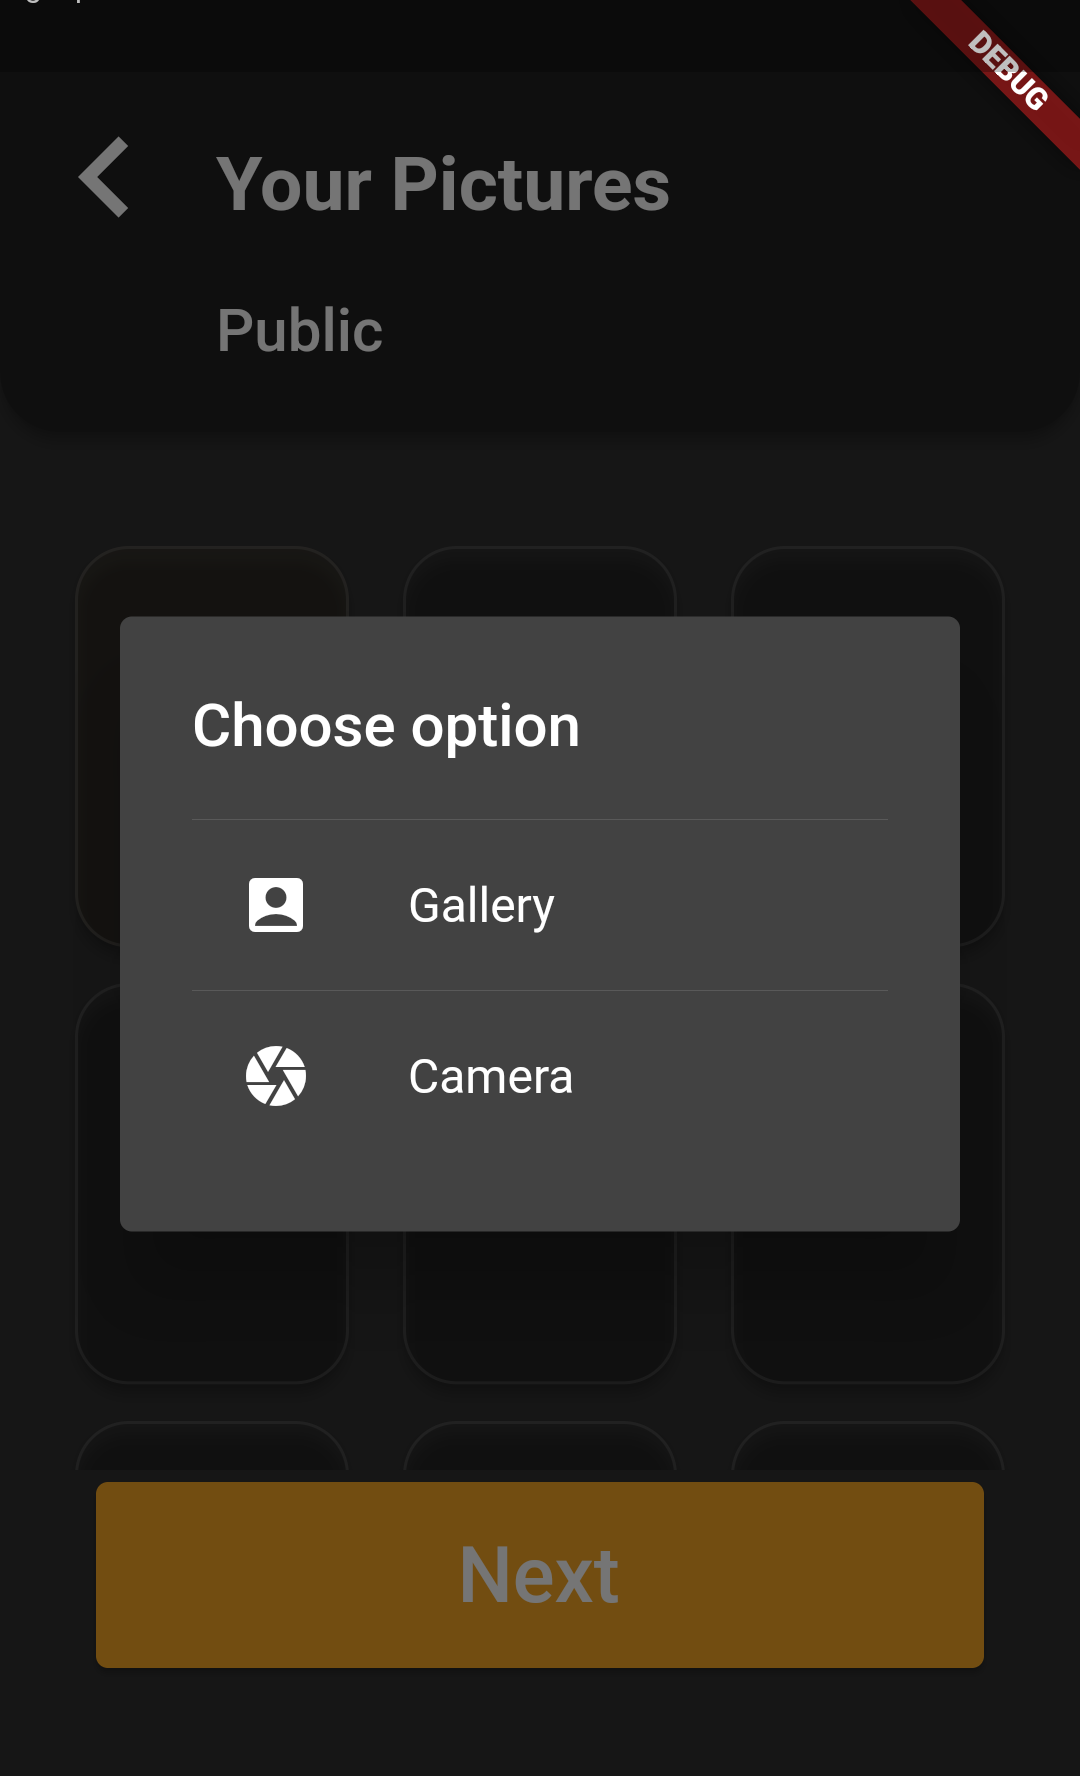
\includegraphics[height=7.7cm,keepaspectratio]{assets/images/ui/signup/18-public-pictures-dialog.png}
		\caption{Public Picture Dialog}
	\end{minipage}\quad
	\begin{minipage}{.45\textwidth}
		\centering
		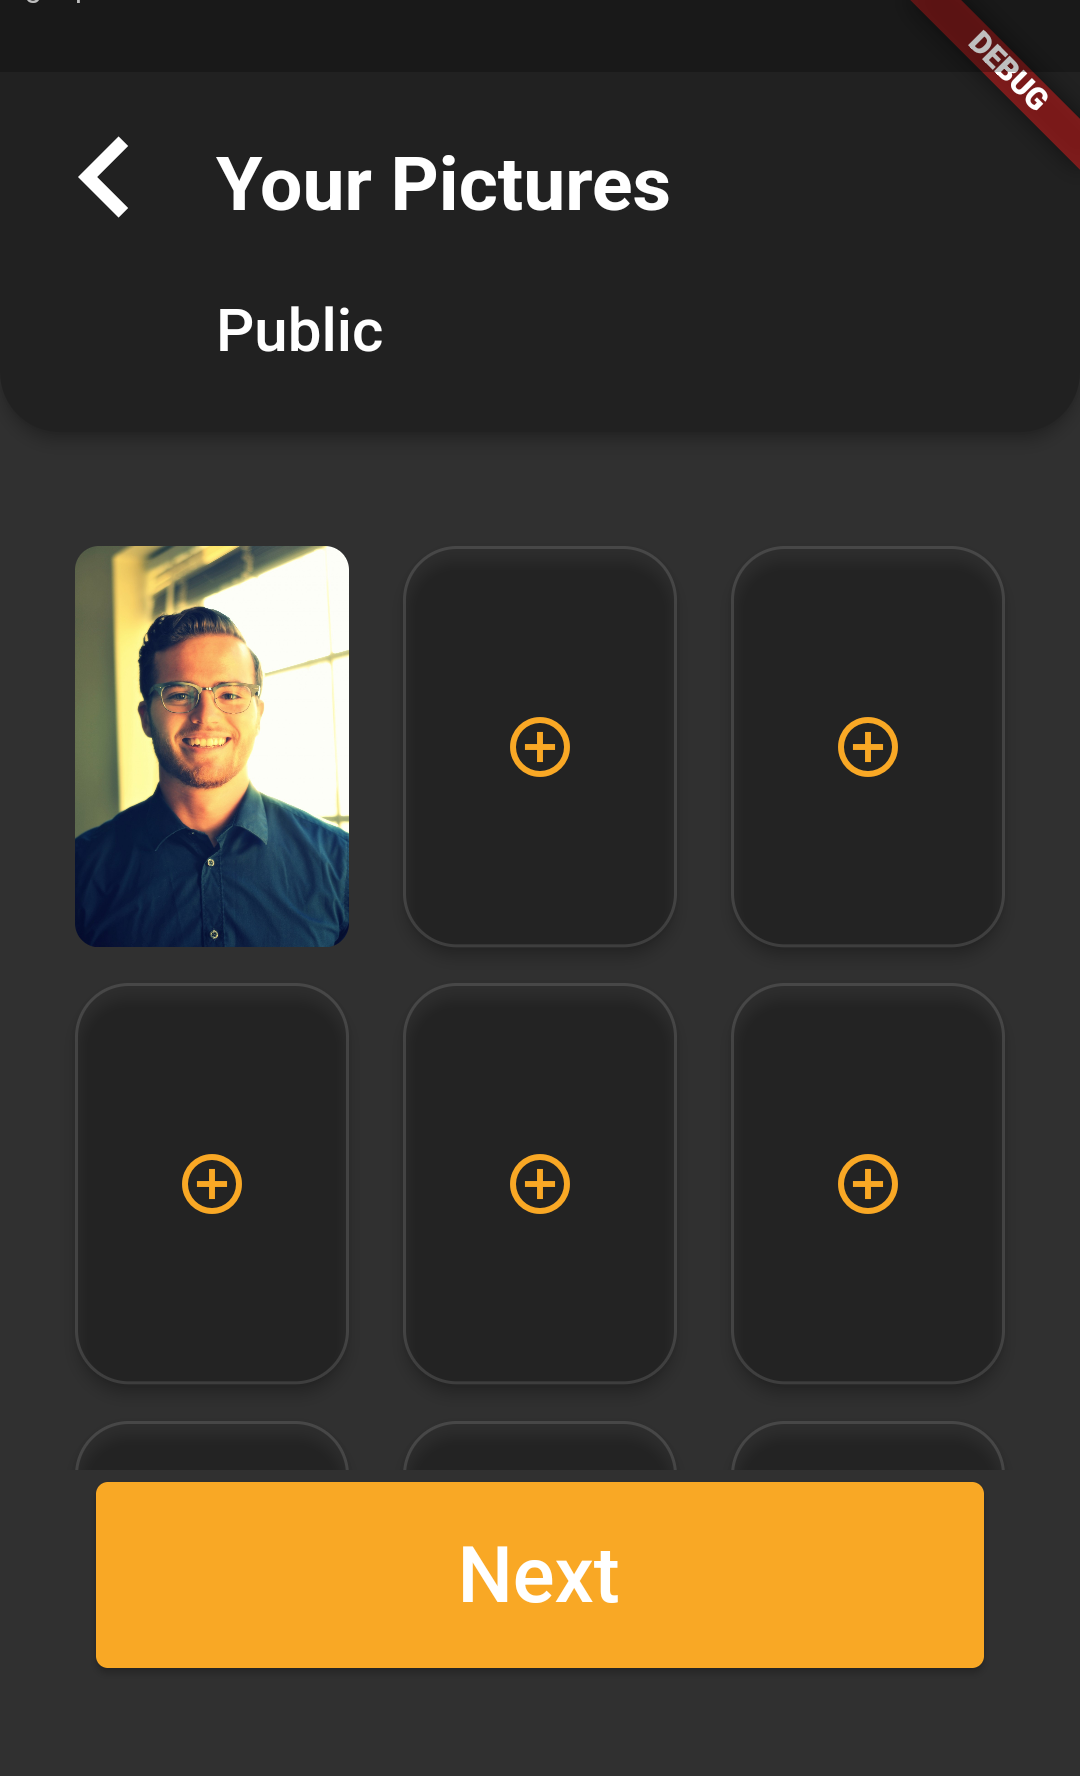
\includegraphics[height=7.7cm,keepaspectratio]{assets/images/ui/signup/19-public-pictures-selected.png}
		\caption{Public Picture}
	\end{minipage}
\end{figure}
\begin{figure}[!htb]
	\centering
	\begin{minipage}{.45\textwidth}
		\centering
		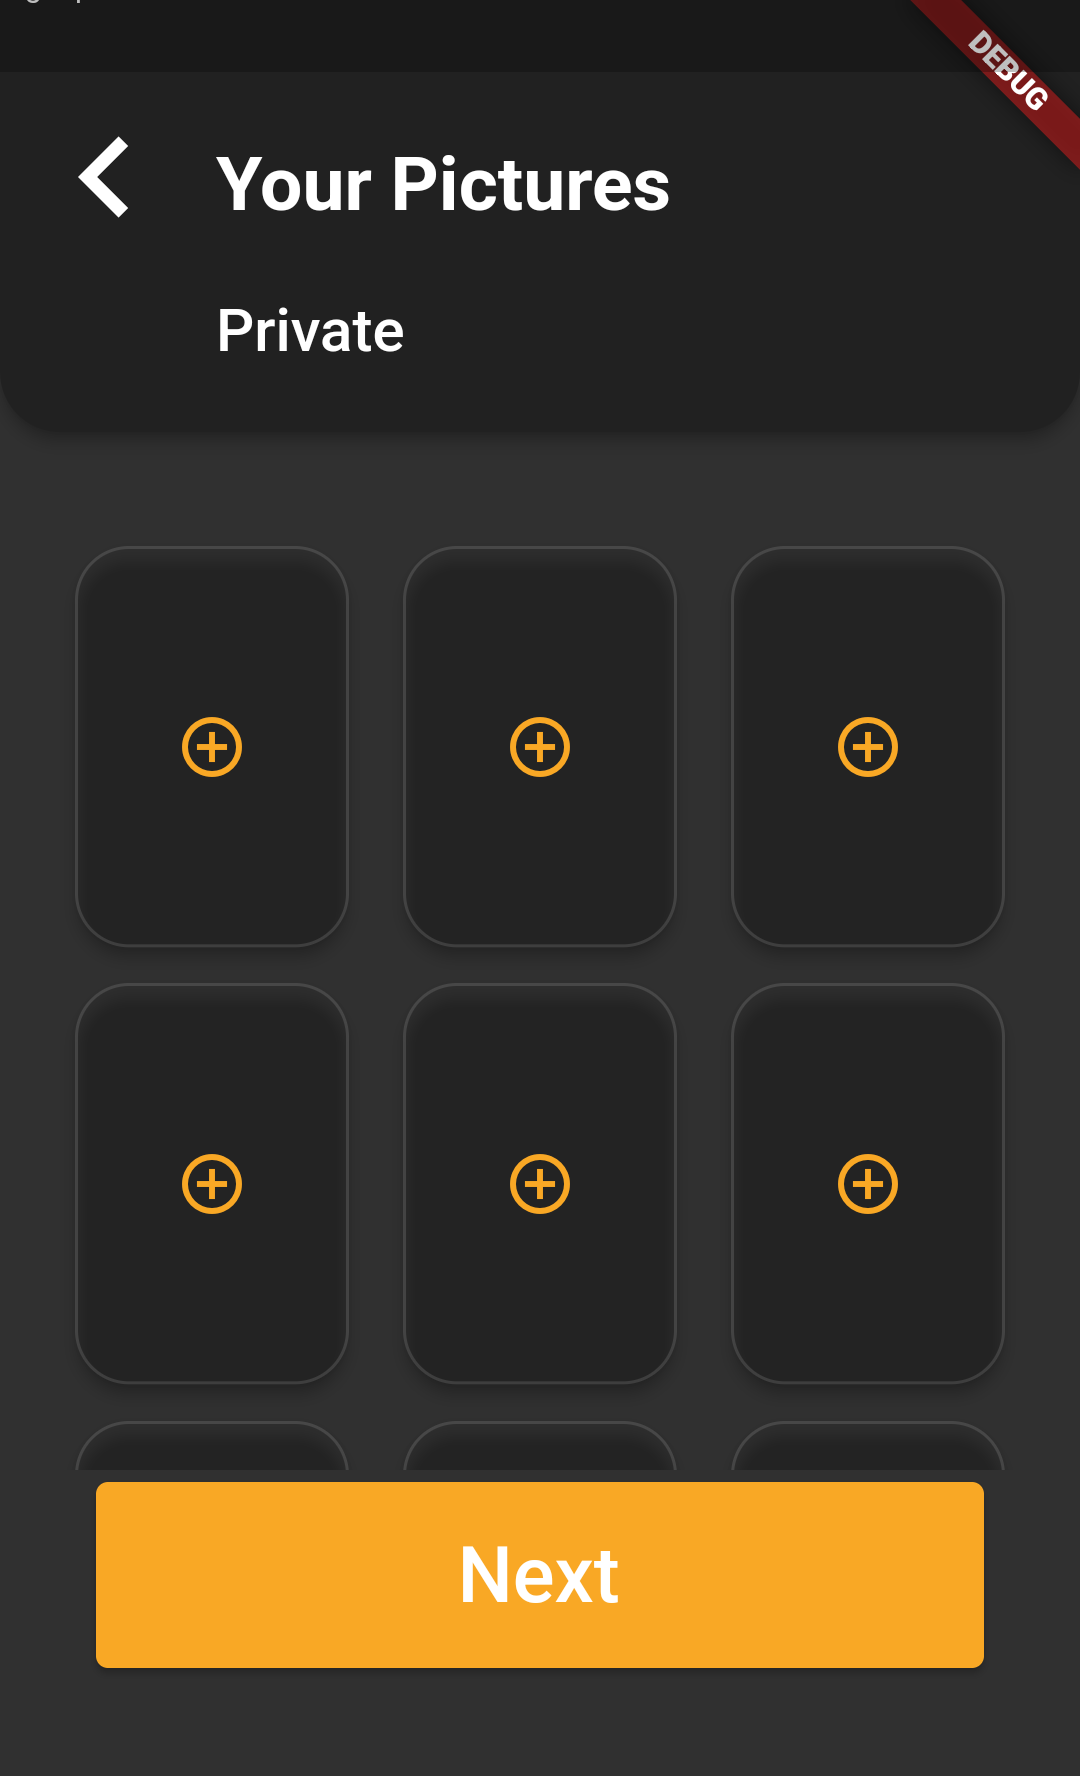
\includegraphics[height=7.7cm,keepaspectratio]{assets/images/ui/signup/20-private-pictures.png}
		\caption{Private Picture Empty}
	\end{minipage}\quad
	\begin{minipage}{.45\textwidth}
		\centering
		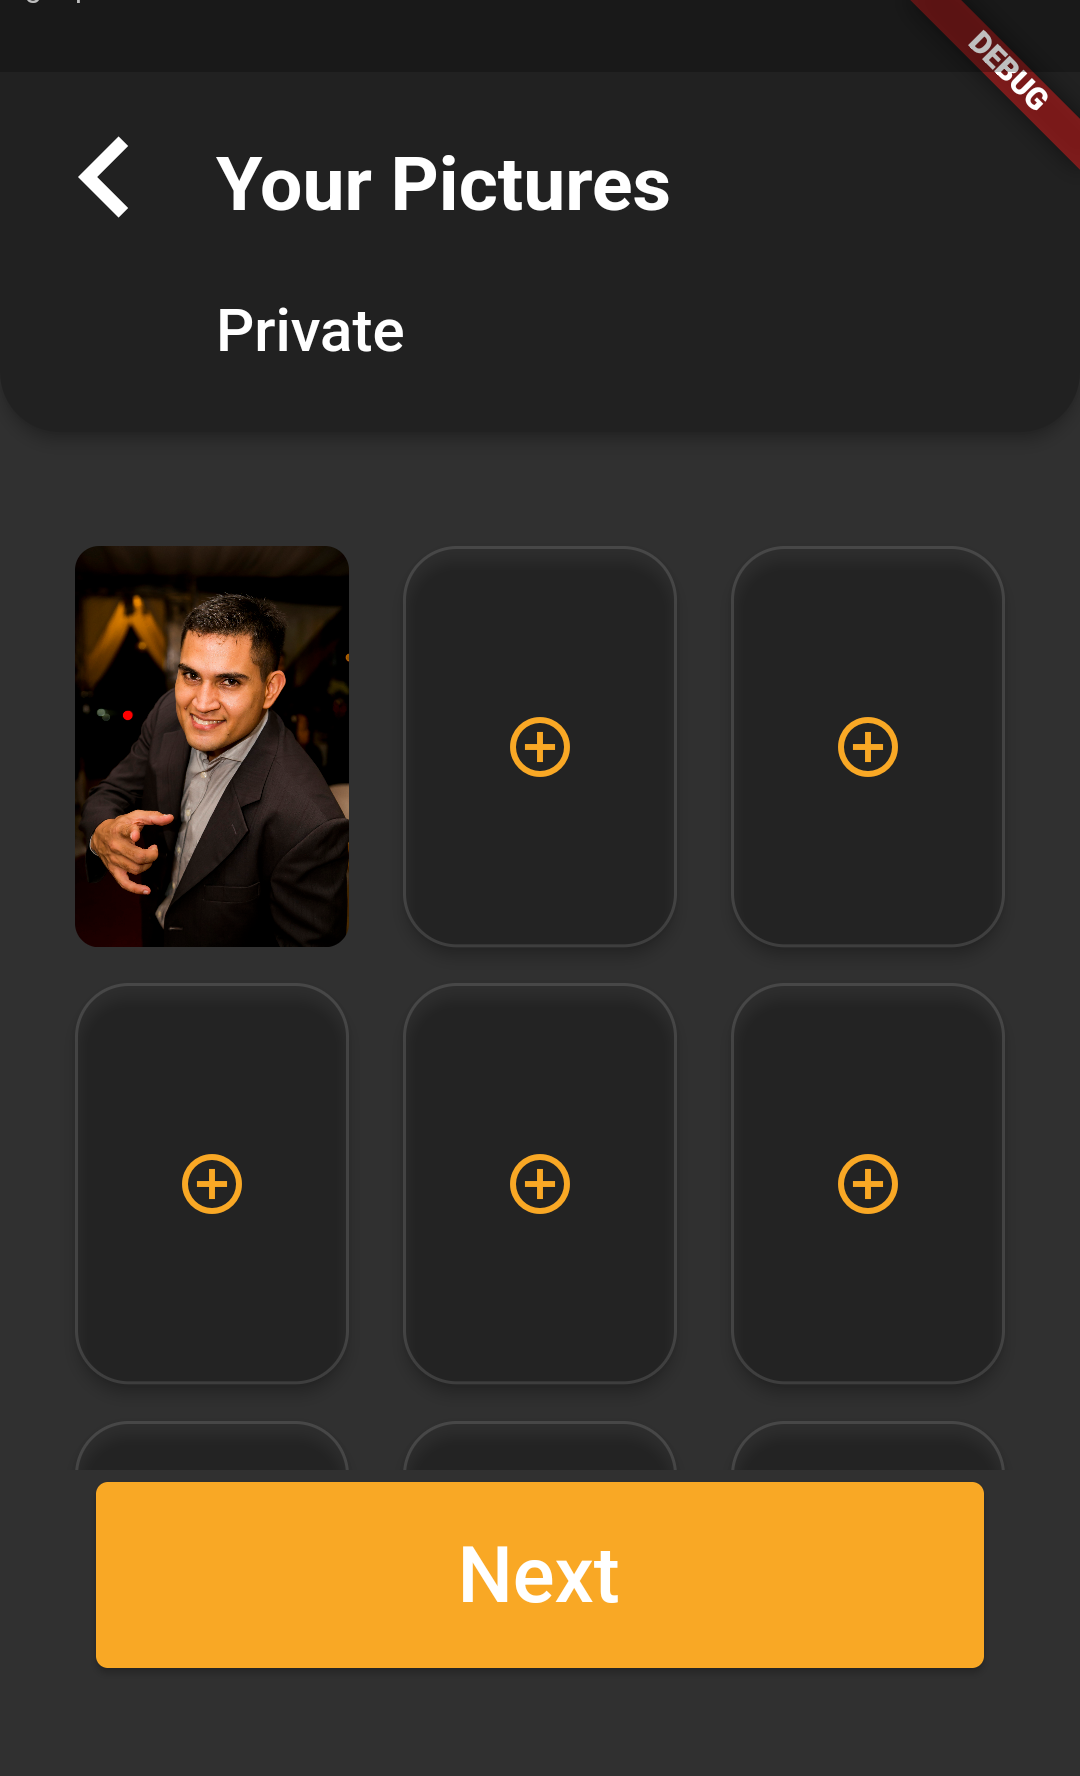
\includegraphics[height=7.7cm,keepaspectratio]{assets/images/ui/signup/22-private-pictures-selected.png}
		\caption{Private Picture}
	\end{minipage}
\end{figure}


\clearpage


\subsubsection{Discover}
\begin{figure}[!htb]
	\centering
	\begin{minipage}{.45\textwidth}
		\centering
		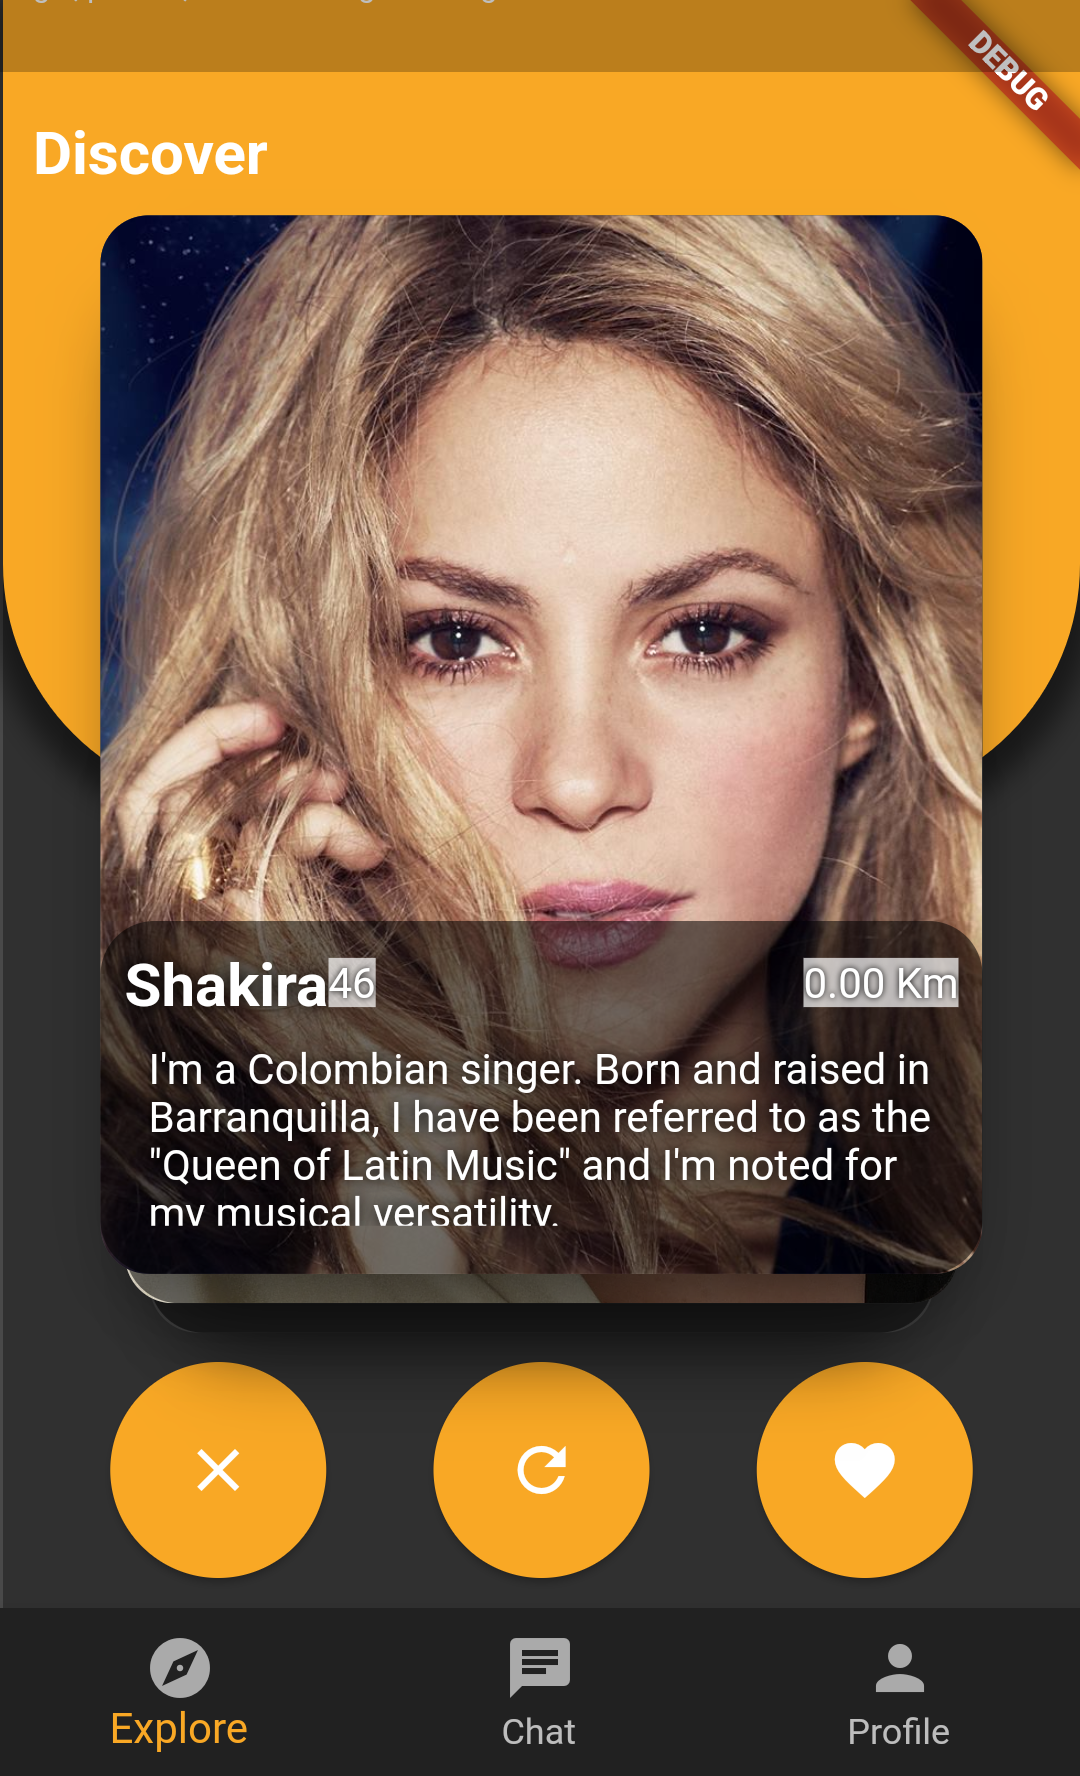
\includegraphics[height=7.7cm,keepaspectratio]{assets/images/ui/discover/03-discover-screen-match-animation.png}
		\caption{Discover}
	\end{minipage}\quad
	\begin{minipage}{.45\textwidth}
		\centering
		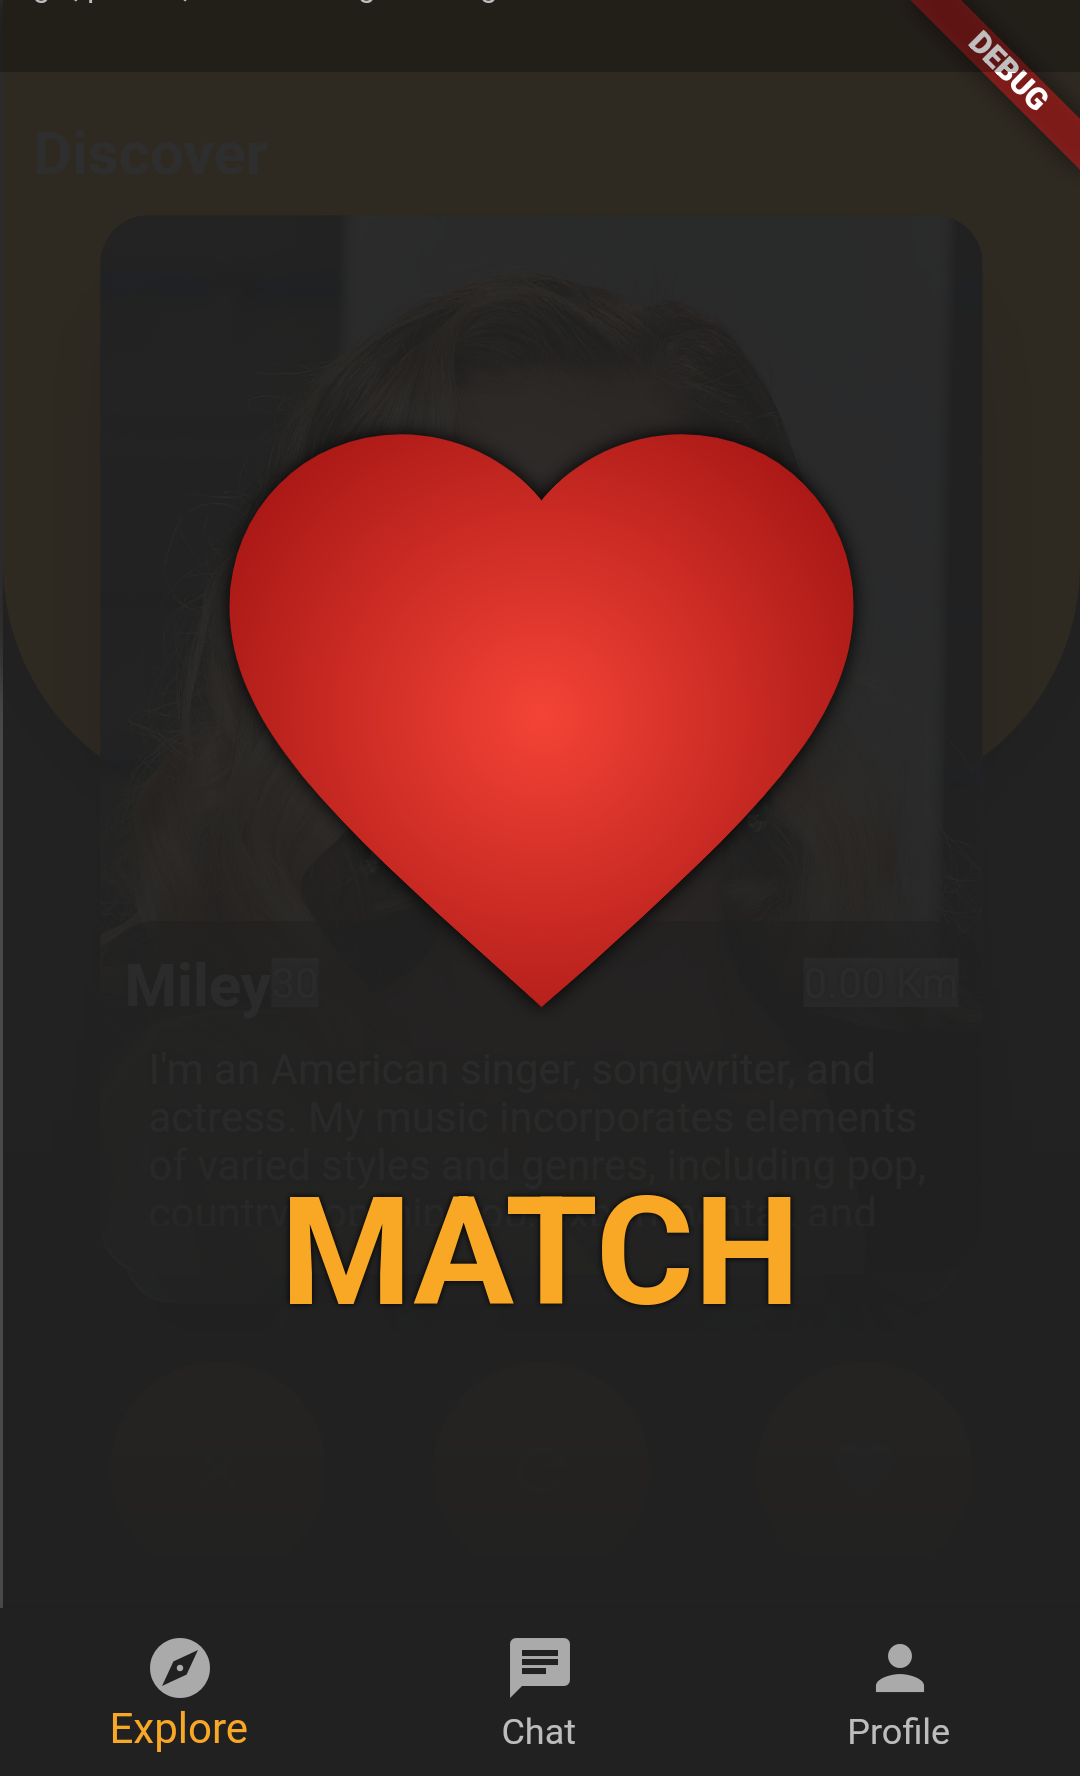
\includegraphics[height=7.7cm,keepaspectratio]{assets/images/ui/discover/06-discover-screen-match-animation.png	}
		\caption{Discover Animation}
	\end{minipage}
\end{figure}
\begin{figure}[!htb]
	\centering
	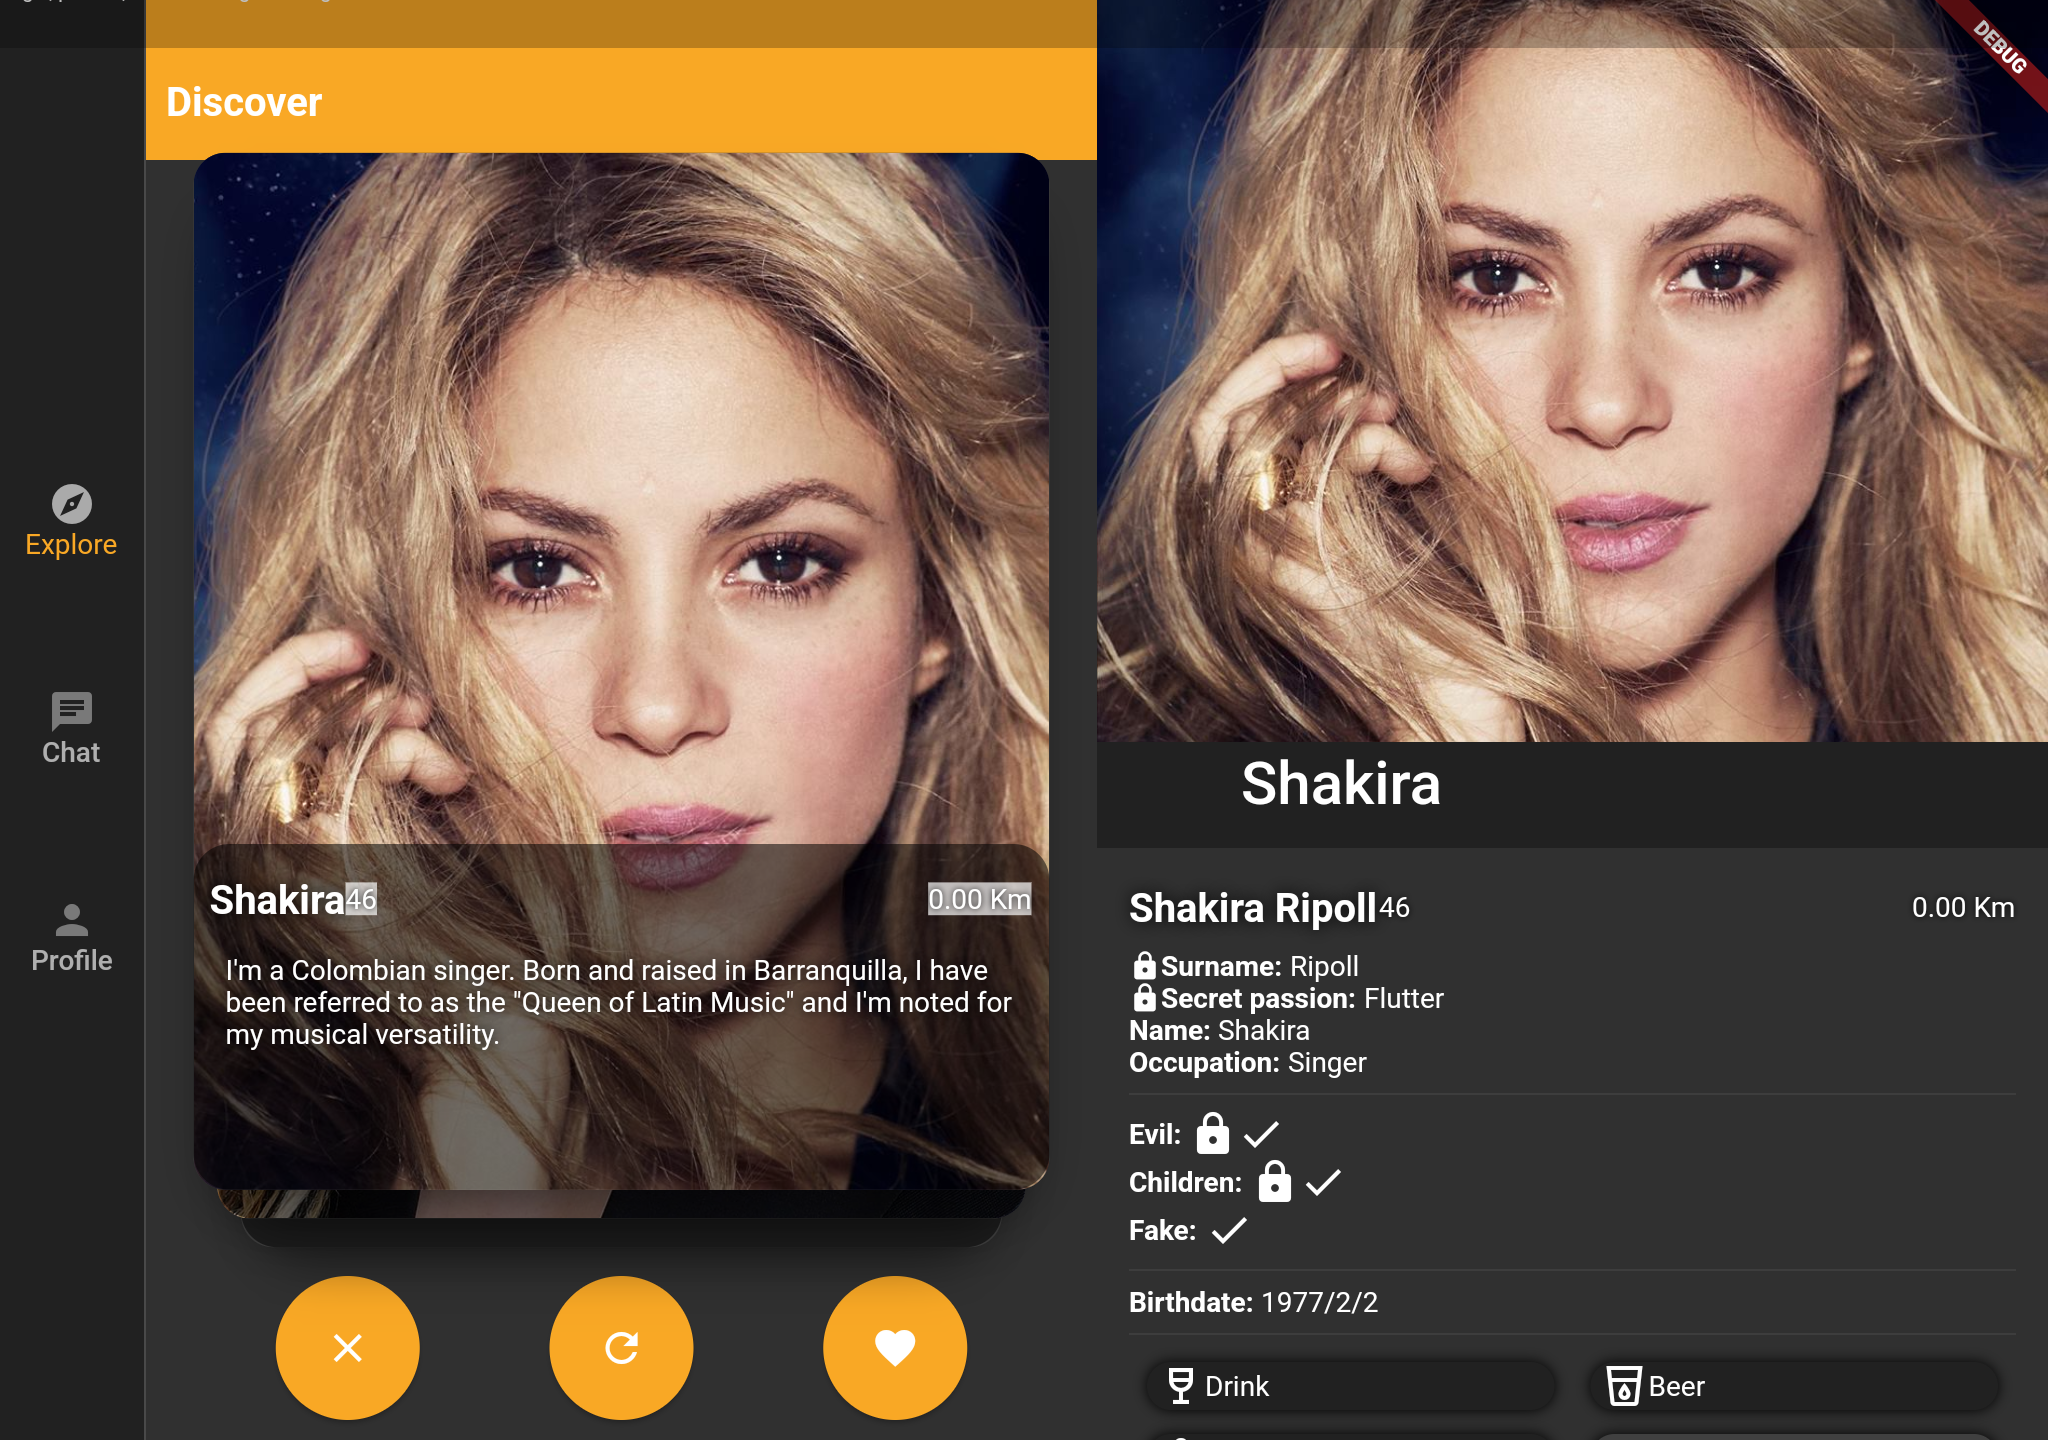
\includegraphics[width=0.8\textwidth]{assets/images/ui/discover/tabler-discover-screen.png}
	\caption{Tablet Discover}
\end{figure}

\clearpage


\subsubsection{Partner Detail}
\begin{figure}[!htb]
	\centering
	\begin{minipage}{.45\textwidth}
		\centering
		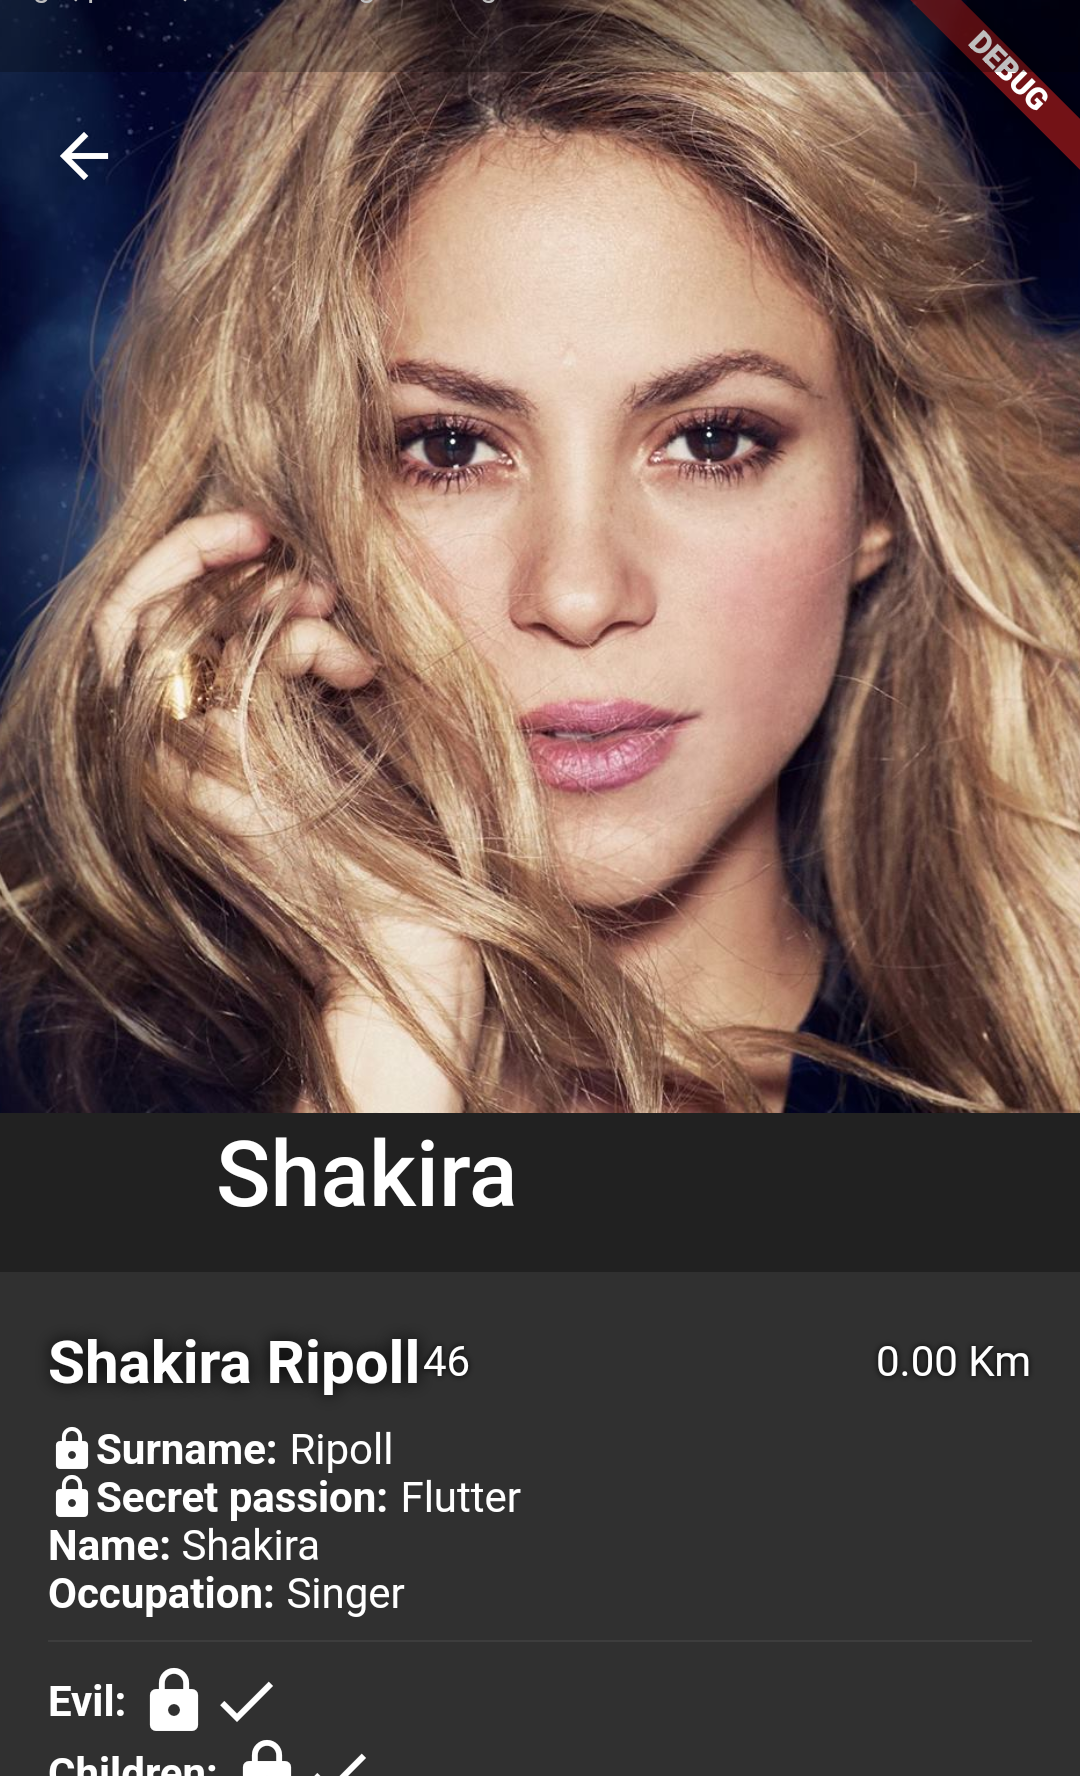
\includegraphics[height=7.7cm,keepaspectratio]{assets/images/ui/partner-detail/14-partner-detail-screen.png}
		\caption{Partner Detail}
	\end{minipage}\quad
	\begin{minipage}{.45\textwidth}
		\centering
		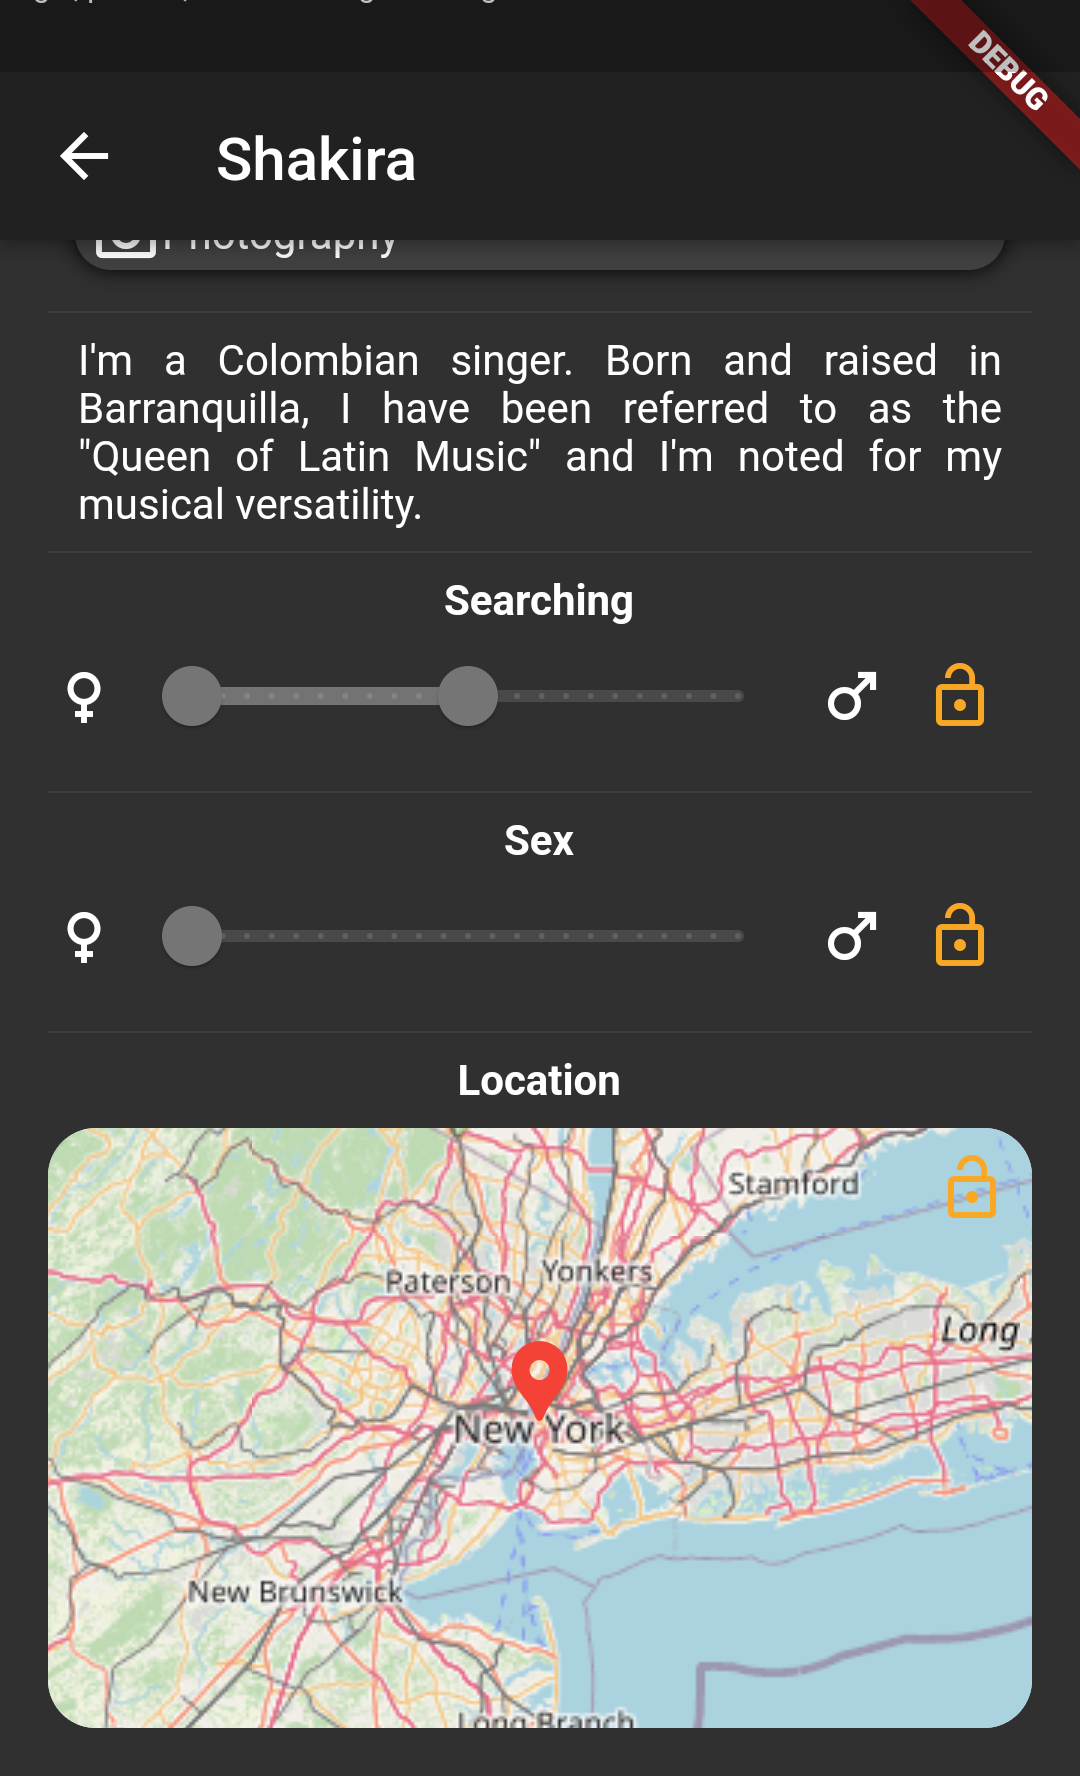
\includegraphics[height=7.7cm,keepaspectratio]{assets/images/ui/partner-detail/15-partner-detail-screen-2.png}
		\caption{Partner Detail Bottom}
	\end{minipage}
\end{figure}

\clearpage
\subsubsection{Chat}
\begin{figure}[!htb]
	\centering
	\begin{minipage}{.45\textwidth}
		\centering
		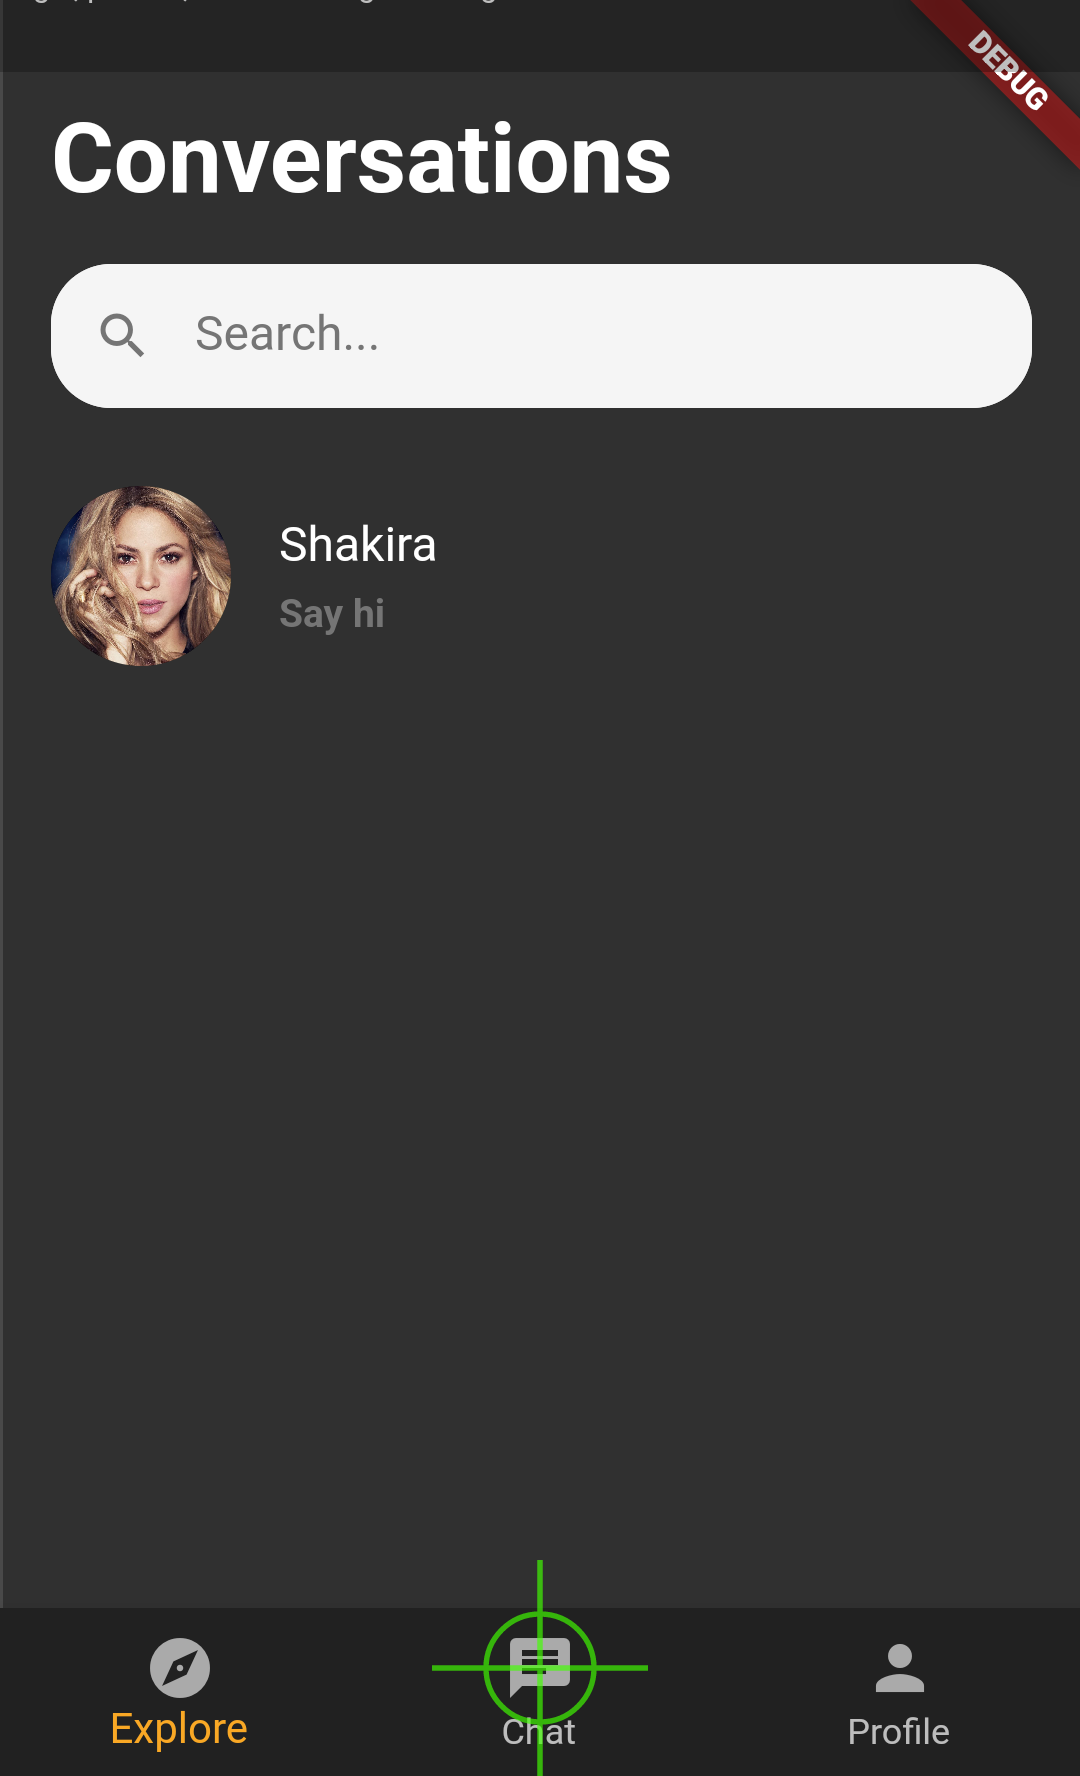
\includegraphics[height=7.7cm,keepaspectratio]{assets/images/ui/chat/10-chat-screen.png}
		\caption{Chat List}
	\end{minipage}\quad
	\begin{minipage}{.45\textwidth}
		\centering
		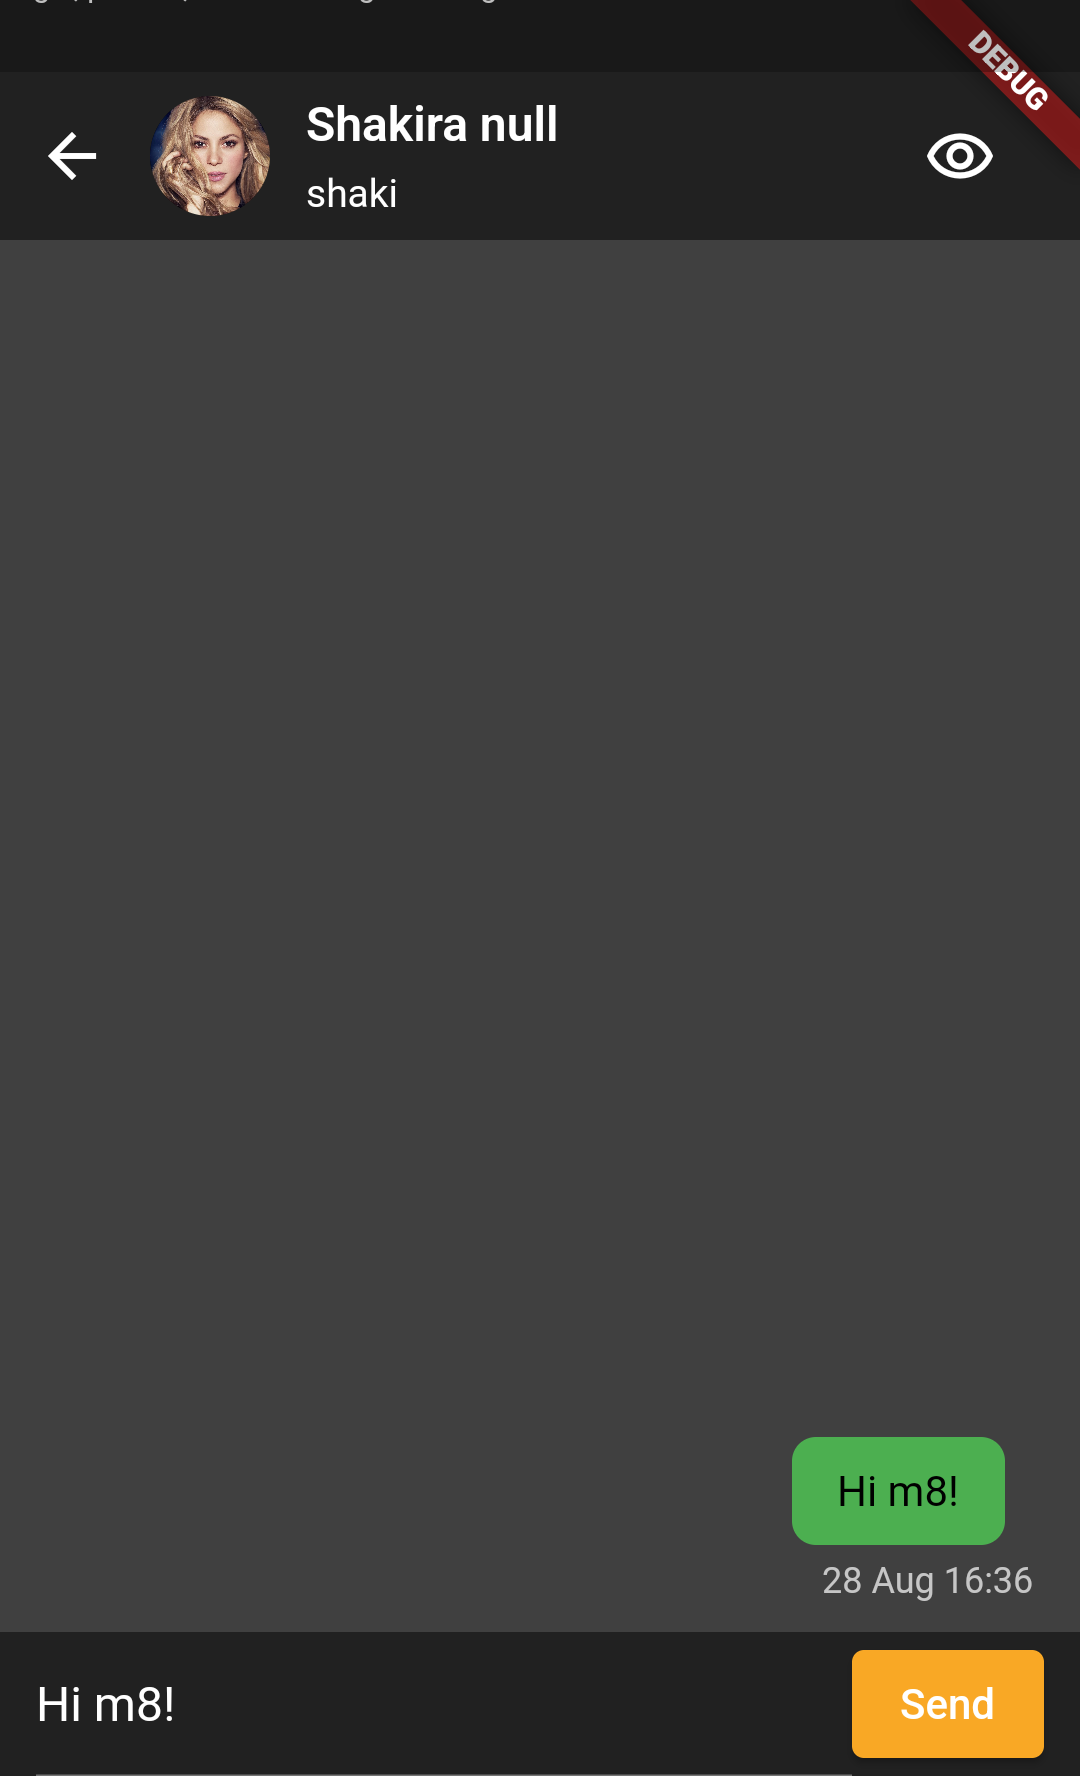
\includegraphics[height=7.7cm,keepaspectratio]{assets/images/ui/chat/13-send-a-message-sent.png}
		\caption{Single Chat}
	\end{minipage}
\end{figure}
\begin{figure}[!htb]
	\centering
	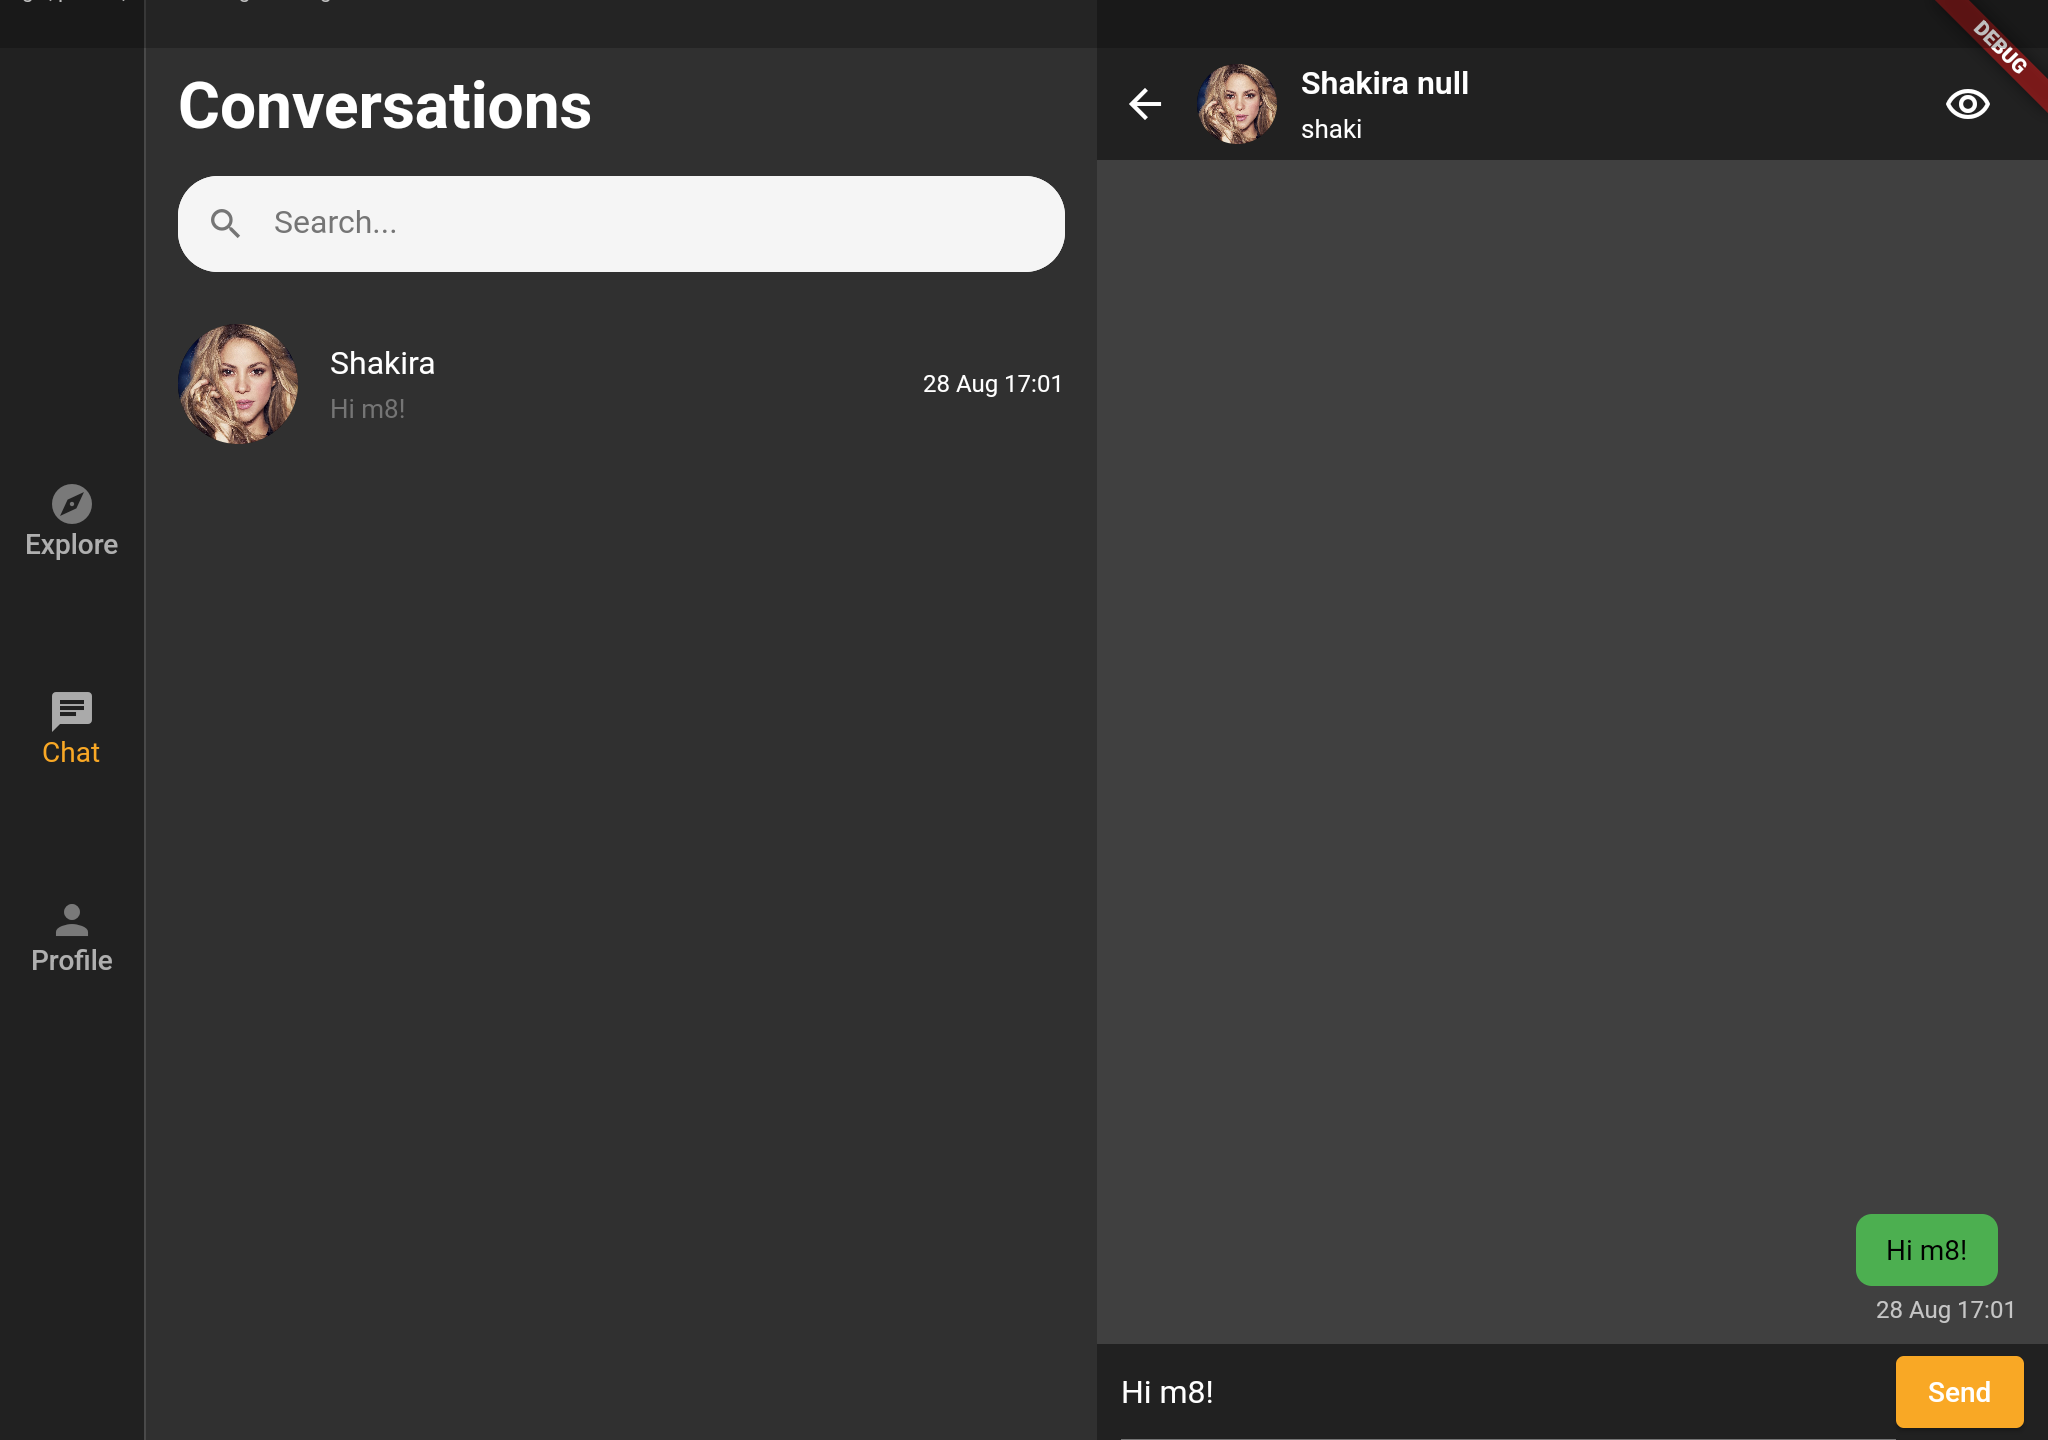
\includegraphics[width=0.8\textwidth]{assets/images/ui/chat/tablet-chat.png}
	\caption{Tablet Chat}
\end{figure}

\clearpage
\subsubsection{Profile}
\begin{figure}[!htb]
	\centering
	\begin{minipage}{.45\textwidth}
		\centering
		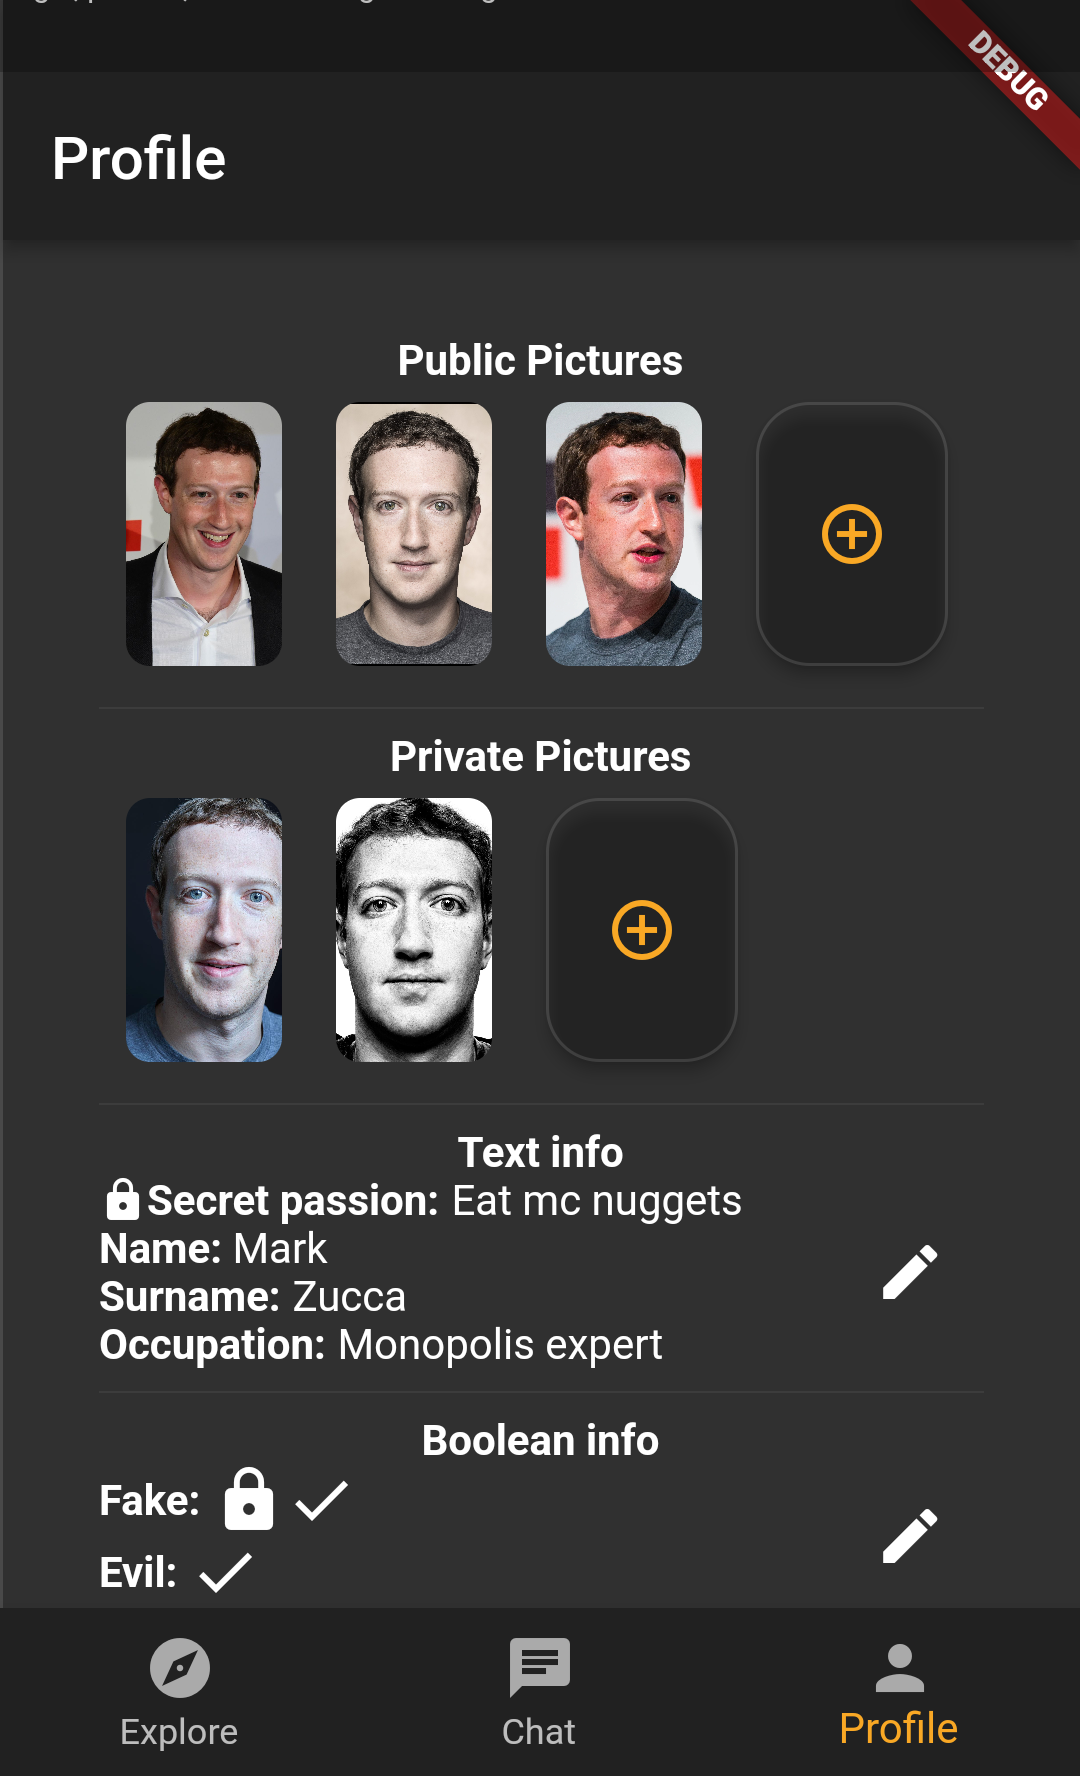
\includegraphics[height=7.7cm,keepaspectratio]{assets/images/ui/profile/18-profile-screen.png}
		\caption{Profile}
	\end{minipage}\quad
	\begin{minipage}{.45\textwidth}
		\centering
		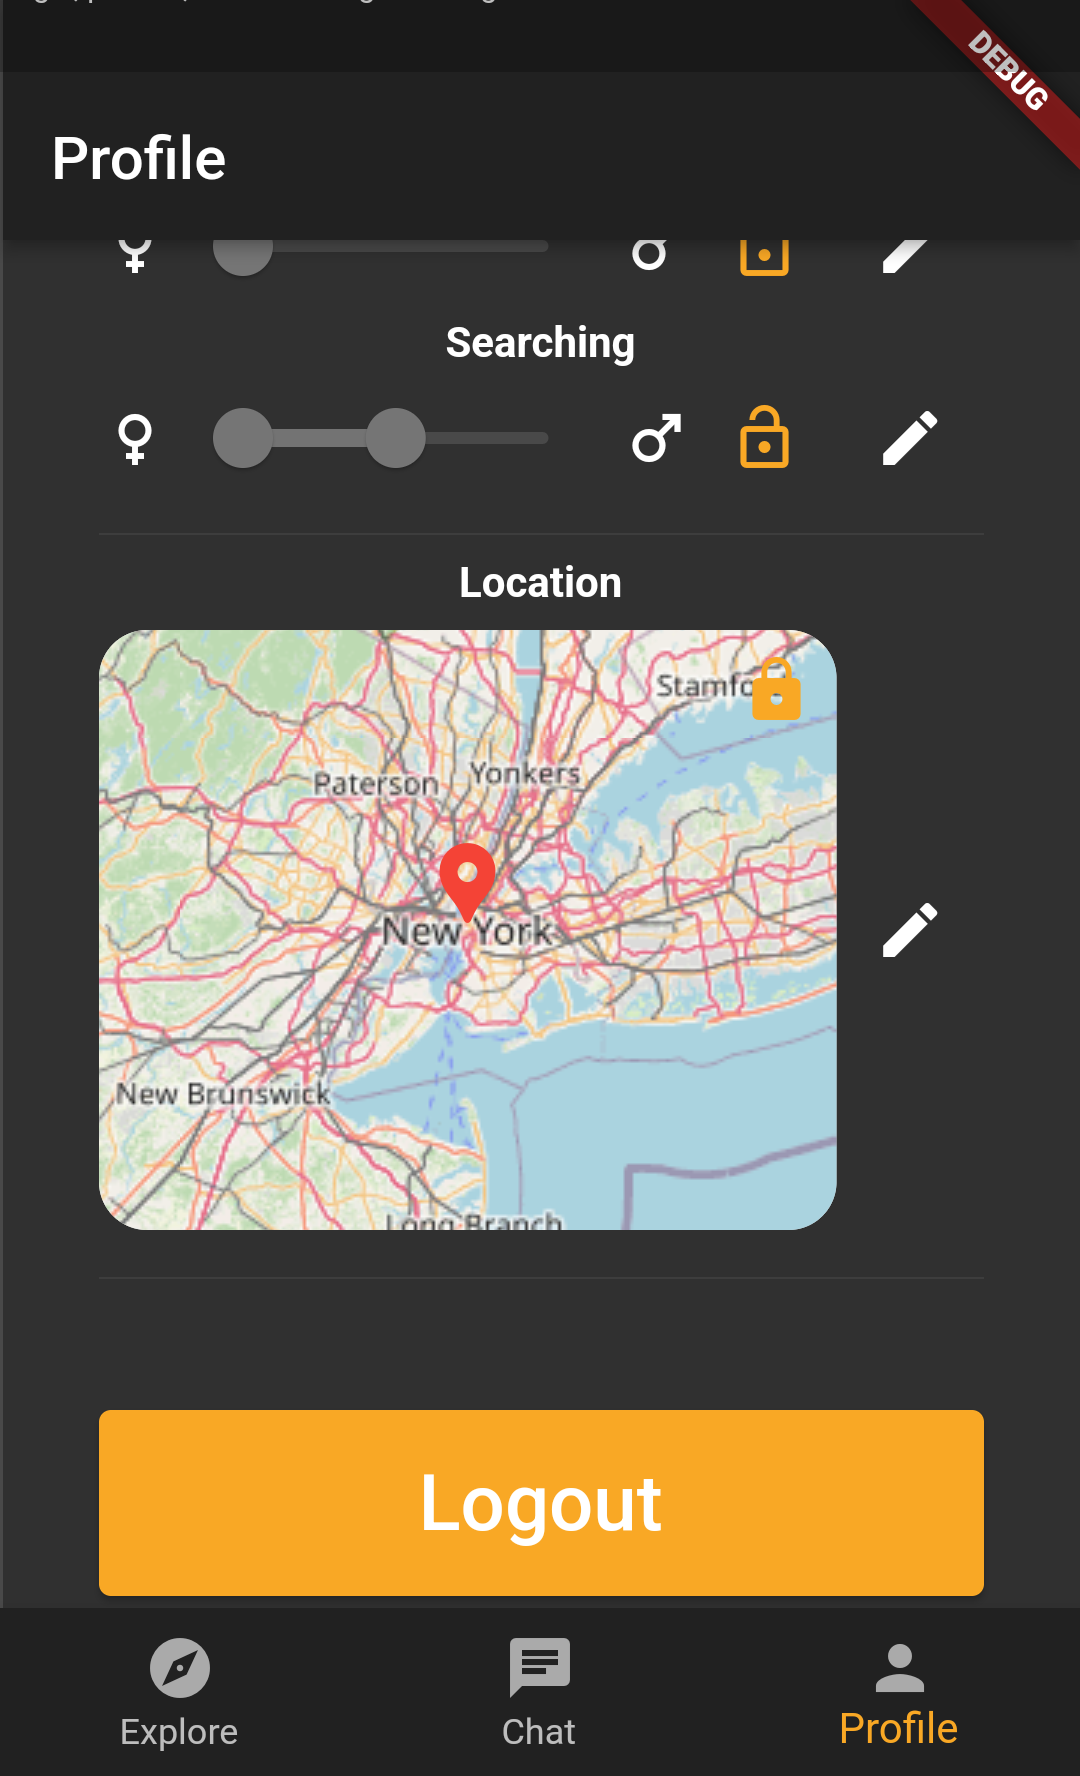
\includegraphics[height=7.7cm,keepaspectratio]{assets/images/ui/profile/19-profile-screen-2.png}
		\caption{Profile Bottom}
	\end{minipage}
\end{figure}
\begin{figure}[!htb]
	\centering
	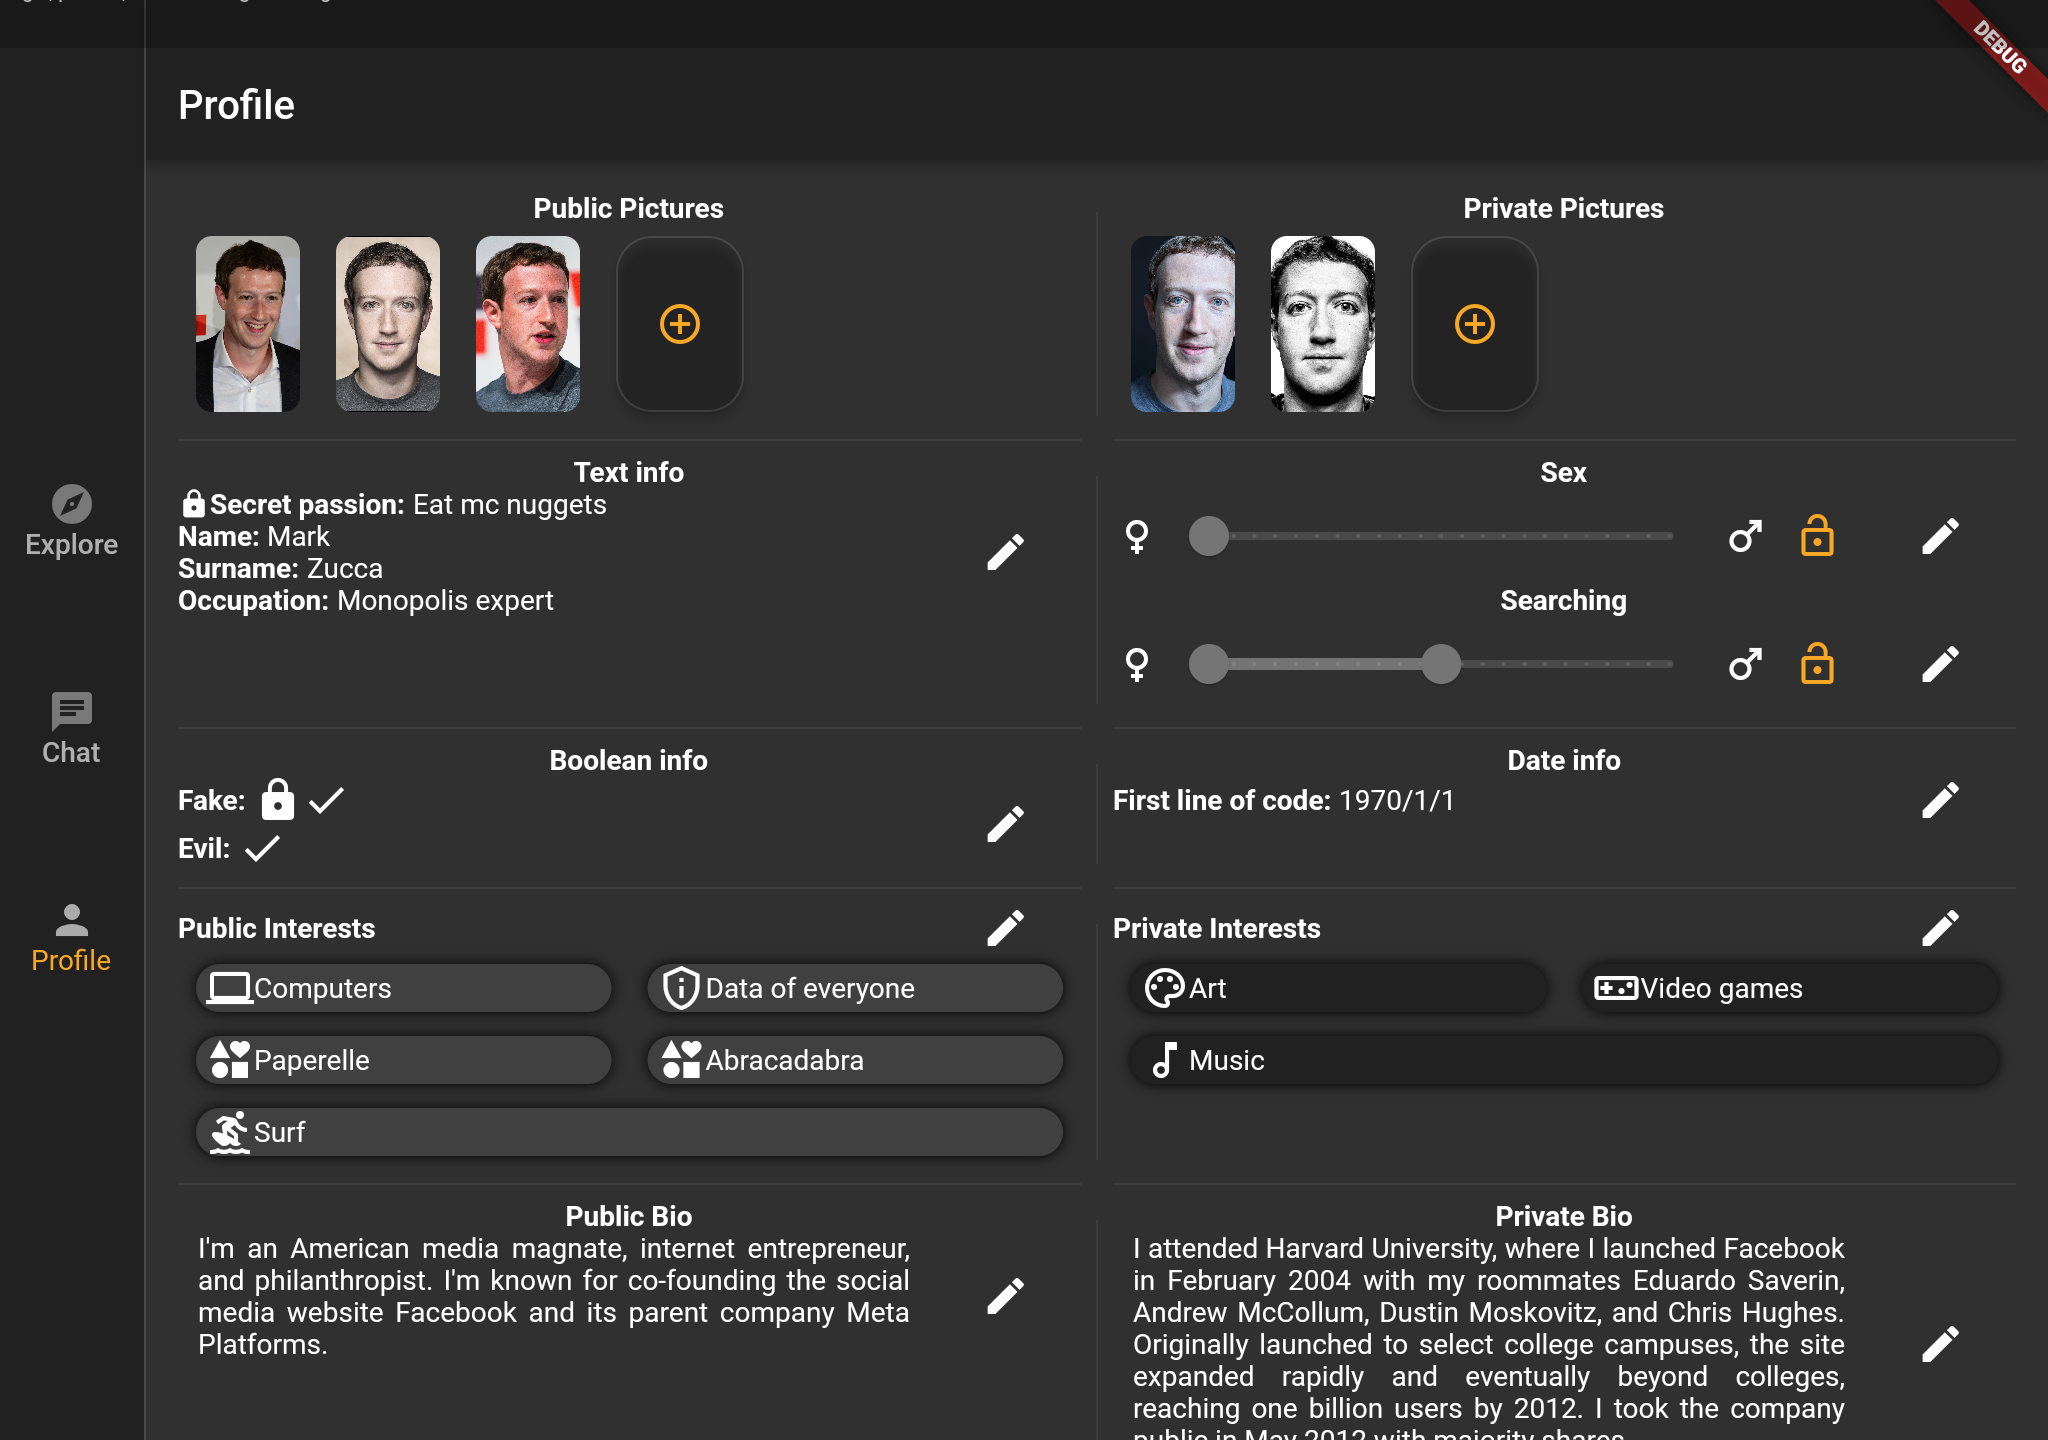
\includegraphics[width=0.8\textwidth]{assets/images/ui/profile/tabler-profile-screen.png}
	\caption{Tablet Profile}
\end{figure}

\clearpage


\section{Implementation, integration and test plan}
\label{sec:ittp}

\subsection{Integration Process}
To develop the app we exploited \textbf{git} with \textbf{Gitlab} that gave us some really useful functionalies. \\
First of we organized the repository in branches:
\begin{itemize} 
	\item \textbf{main} \\
		Where only the releases will be merged.
	\item \textbf{development} \\
		Where there is the actual state of the developed app.
	\item \textbf{feature-branches} \\
		Any time we want to add a feature, we create a branch from development and merge in development when the feature is ready.
\end{itemize} 
This organization make possible to use the CI of gitlab, we configured it to run all the tests and make a report every time we open a Merge Request.
The gitlab UI doesn't let you merge untill the tests are all passed avoiding the merge of code that may contain bug.
\begin{figure}[!htb]
	\centering
	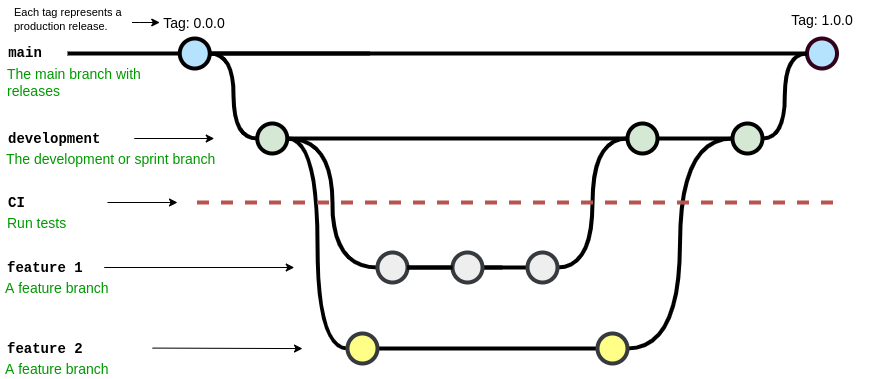
\includegraphics[width=1\textwidth]{assets/images/git-ci.drawio.png}
	\caption{Git CI}
\end{figure}

\newpage

We also exploited \textbf{Lefthook} a git hooks manager to: 
\begin{itemize} 
	\item Allow only commit that respect the Conventional Commits standard. 
	\item Run `dart fix` to fix all the autamatically fixable lint problem and `flutter format` that format the code to follow the code style choosen.
	\item When try to push run the tests and the analyzer and block the push if one fail.
\end{itemize} 
\vspace*{1cm}

To help us write cleaner code we imported \href{https://pub.dev/packages/very_good_analysis}{Very Good Analysis} that provides with a lot of lint rules.

\newpage
\subsection{Testing}

\subsubsection{Unit testing}
We have tested every component of the app with Unit Testing reaching a coverage of around \textbf{95\%}. \\
We have around 400 tests and widget tests.

\begin{figure}[!htb]
	\centering
	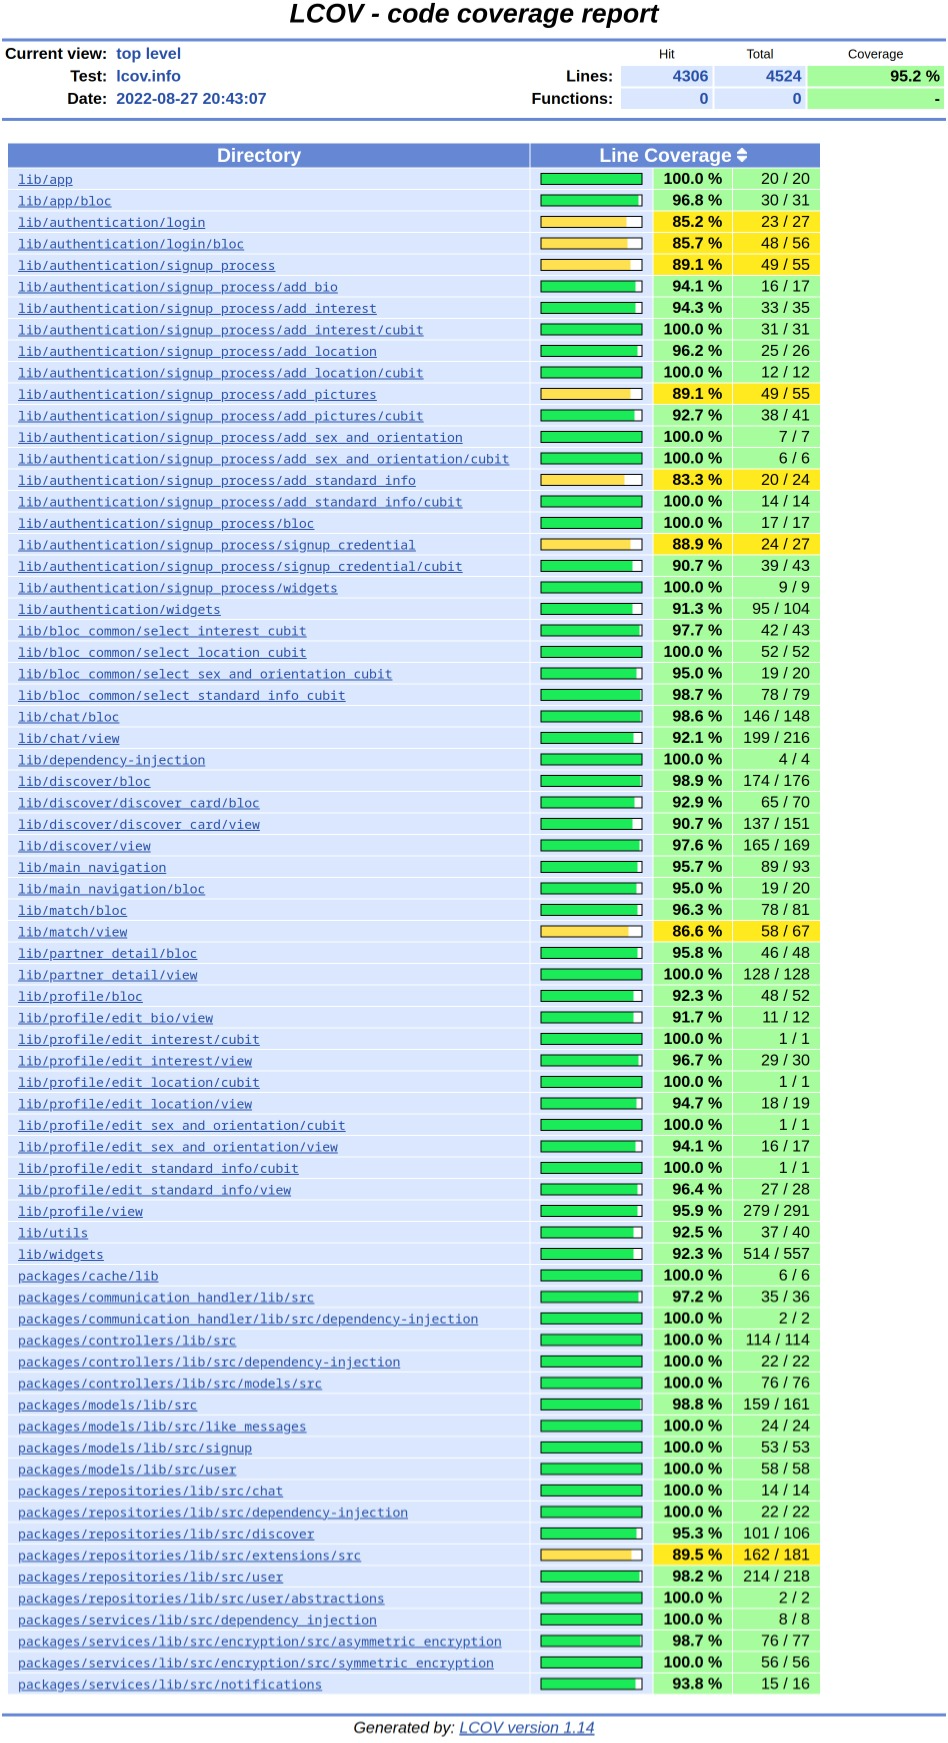
\includegraphics[width=0.65\textwidth]{assets/images/lcov-report.png}
	\caption{Coverage}
\end{figure}
\clearpage
To make possible to run the tests we explited some components:
\begin{itemize} 
	\item An adaptation this \href{https://github.com/brianegan/flutter_architecture_samples/blob/master/scripts/runTests.sh}{script} that made possible to run all the tests from the packages and lib folder and than merge the lcov.info files generate from the different packages in a single one.
	\item \texttt{genhtml} to generate the html report from the lcov.info file
	\item \texttt{cobertura} to convert the lcov.info report to cobertura format readable by gitlab
	\item \texttt{Mocktail} to make it easy to mock the components not under test
\end{itemize} 

\subsubsection{Integration testing}
We also implemented a couple of integretion test that help to identify regression bug when a new feature is introduced.
\begin{itemize} 
	\item \textbf{Signup} \\ that make a complete signup process navigating through all the nine screen of the signup flow submitting fake data and landing in the Discover page. It also take screenshots to every screen that it pass through for later analysis.
	\item \textbf{Login, put like, send message and logout}  \\ Execute those steps:
		\begin{itemize} 
			\item Do the login landing in the Discover page.
			\item Put a like to the first partner visible getting a match animation.
			\item Navigate to the Chat screen.
			\item Open the conversation with the matched partner.
			\item Send a message.
			\item Open the PartnerDetail page and scroll untill it reach the bottom.
			\item Close the PartnerDetail page and conversation.
			\item Navigate to the Profile page and scroll down.
			\item Make a logout landing in the Login page.
		\end{itemize}
\end{itemize} 

\subsubsection{Other types of testing}
Other than that we spent some time to manually test the app. Trying to find edge cases where it could broke.

\newpage
\section{References}
\begin{itemize}
	\item \href{https://flutter.dev/}{Flutter}
	\item \href{https://github.com/felangel/mocktail/tree/main/packages/mocktail/}{Mocktail}
\end{itemize}
\subsection{Software used for this document}
\begin{itemize}
	\item \href{https://www.draw.io/}{Draw.io}: Diagrams
	\item \href{https://www.latex-project.org/}{LaTeX}: Document preparation system 
	\item \href{https://vscodium.com/}{VSCodium}: Text Editor with user-friendly live share plugin
\end{itemize} 

\end{document}